\documentclass{kul-ulille-beamer}
%\setbeameroption{show notes on second screen=right} % Both


%% Preamble ===================================================================
\usepackage{defense}



% Meta ========================================================================
\addbibresource{references.bib}

\title{%
  A visual Brain-Computer Interface \\
  for gaze-free communication
}
\author{Arne Van Den Kerchove}
\date{December 16, 2024}

\begin{document}
% =============================================================================

\titleframe

% =============================================================================

\begin{frame}
  \frametitle{The Locked-in Syndrome}
  \centering
  \begin{minipage}[c]{.4\textwidth}
    \small
    \raggedright
    Complete paralysis, \\ \emph{impaired communication}
    \bigskip

    Due to
    \begin{itemize}
      \item Stroke
      \item Traumatic brain injury
      \item Neurodegenerative diseases
      \item \ldots
    \end{itemize}
    \bigskip

  Assistive technology
  \bigskip

  A Brain-Computer Interface (BCI) bypasses muscle activity

 \end{minipage}\hfill%
  \begin{minipage}[c]{.5\textwidth}
    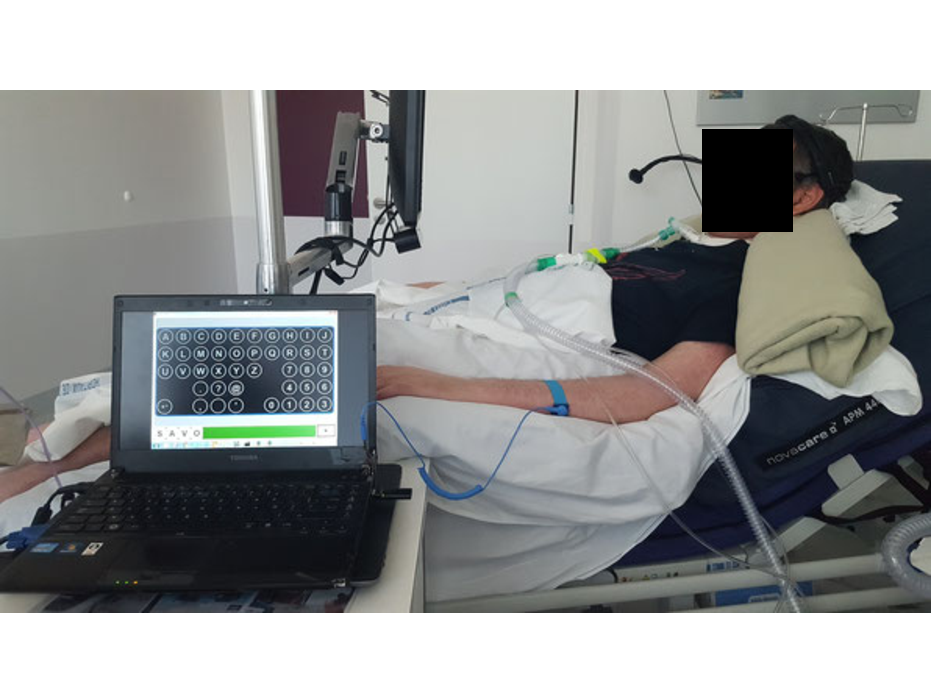
\includegraphics[width=\textwidth]{figures/intro/damien.pdf}
  \end{minipage}
\end{frame}
\begin{frame}[noframenumbering]
  \frametitle{The Locked-in Syndrome}
  \centering
  \begin{minipage}[c]{.4\textwidth}
    \small
    \raggedright
    Complete paralysis, \\ \emph{impaired communication}
    \bigskip

    Due to
    \begin{itemize}
      \item Stroke
      \item Traumatic brain injury
      \item Neurodegenerative diseases
      \item \ldots
    \end{itemize}
    \bigskip

  Assistive technology
  \bigskip

    A \emph{Brain-Computer Interface} (BCI) bypasses muscle activity

 \end{minipage}\hfill%
  \begin{minipage}[c]{.5\textwidth}
    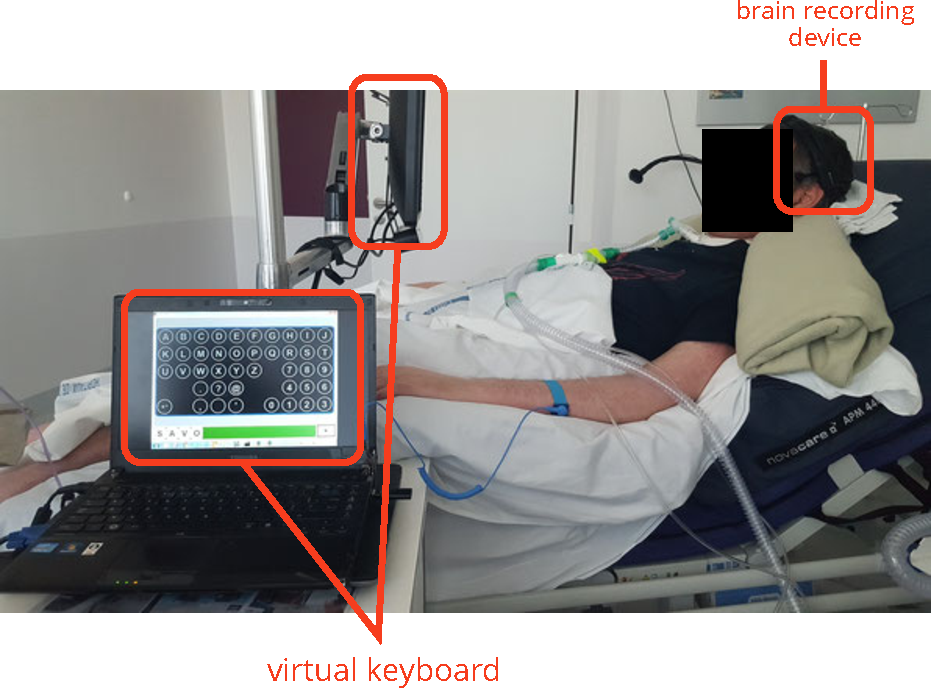
\includegraphics[width=\textwidth]{figures/intro/damien_annot.pdf}
  \end{minipage}
\end{frame}



\begin{frame}
  \frametitle{The Brain-Computer Interface}
  \schema{figures/intro/bci.pdf}
\end{frame}


\begin{frame}[c]
  \frametitle{Research question}
  \centering

  \begin{minipage}{.8\textwidth}
  \centering
  \huge
  How can we optimize \emph{BCI}  assistive technology design  to make it more
    \emph{efficient} and  \emph{accessible}?
  \end{minipage}

\end{frame}


% =============================================================================

\outline{Outline}{figures/outline_design.pdf}
{
  \setbeamercolor{background canvas}{bg=mylightgray}
  \begin{frame}[noframenumbering]
  \frametitle{Outline}
    \schema{figures/outline.pdf}
  \end{frame}
}

\begin{frame}[c]
  \frametitle{Recording the brain activity}
  \schema{figures/intro/recording_modalities.pdf}
  \hfill
  \aside{%
    \emph{EEG}  measures the \\ electrical field on the
    scalp:
    \begin{itemize}
      \item[\textcolor{mygreen}{+}] Non-invasive
      \item[\textcolor{mygreen}{+}] Cheap
      \item[\textcolor{myred}{--}] Large scale activity
      \item[\textcolor{myred}{--}] High noise
    \end{itemize}
    \bigskip

    \ergo Account for this in task and decoder design
  }
\end{frame}



%\begin{frame}[c]
%  \frametitle{BCI paradigms for communication}
%  \begin{minipage}[c]{.5\textwidth}
%    \footnotesize
%    \sffamily
\begin{tikzpicture}[
    scale=\textwidth/3cm,
  ]
  %\useasboundingbox (-1,-1.25) rectangle (1,1);
  \pgfmathsetmacro{\margin}{.1}
  \pgfmathsetmacro{\center}{.5+.5*\margin}
  \pgfmathsetmacro{\textspacing}{.15}
  %\begin{scope}[shift={(1,1.2)}]
    % Draw axes
    \draw[mydarkgray, very thick, <->] ({-(1+\margin)}, 0) -- ({1+\margin},0);
    \draw[mydarkgray, very thick, <->] (0,{-(1+\margin)}) -- (0,{1+\margin});

    % Draw rectangles
    \draw[draw=accent1, fill=white, very thick] ({-\margin}, \margin) rectangle (-1,1);
    \draw[draw=accent2, fill=white, very thick] (\margin, \margin) rectangle (1,1);
    \draw[draw=accent3, fill=white, very thick] (-1, {-\margin}) rectangle (1,-1);

    %% Add text
    \node[color=accent1, align=left,font=\bfseries, anchor=north west, inner sep=2pt] at  (-1,1){active};
    \node[color=accent2, align=left,font=\bfseries, anchor=north east, inner sep=2pt] at  (1,1){reactive};
    \node[color=accent3, align=left,font=\bfseries, anchor=south west, inner sep=2pt] at  (-1,-1){passive};

    \node[color=mydarkgray, align=center,font=\bfseries, anchor=north] at
    (0,{-(1+\margin)}) {passive\\participation};
    \node[color=mydarkgray, align=center,font=\bfseries, anchor=south] at
    (0,{1+\margin}) {active\\participation};
    \node[color=mydarkgray, align=center,font=\bfseries, anchor=east] at ({-(1+\margin)}, 0) {stimulus\\independent};
    \node[color=mydarkgray, align=center,font=\bfseries, anchor=west] at ({1+\margin},0) {stimulus\\dependent};

    %% Text in rectangles
    \node[align=center] at ({-\center}, {\center-\textspacing}) {movement};
    \node[align=center] at ({-\center}, {\center+\textspacing}) {speech};
    %\node[align=center] at ({-\center}, {\center-1.5*\textspacing}) {neurofeedback};

    \node[align=center] at ({\center}, {\center-1.5*\textspacing}) {tactile};
    \node[align=center] at ({\center}, {\center}) {auditory};
    \node[align=center] at ({\center}, {\center+1.5*\textspacing}) {visual};
    %\node[align=center] at ({\center-\textspacing}, {\center-\textspacing}) {mVEP};

    %% More text
    %\node[align=center] at ({\center}, {-\center+\textspacing}) {error\\potentials};
    %\node[align=center] at ({-\center}, {-\center+\textspacing}) {attention and \\ workload detection};
    %\node[align=center] at ({-\center}, {-\center-\textspacing}) {clinical neuroimaging \\ and monitoring};
    %\node[align=center] at ({+\center}, {-\center-\textspacing})  {emotion \\ detection};
    \node[align=center] at (0, {-\center})  {$\cdots$};
  %\end{scope}
\end{tikzpicture}

%  \end{minipage}\hfill%
%
%  \aside{%
%    \small
%    %\emph[accent3]{Passive} BCIs not meant for communication
%      \smallskip
%
%      \emph[accent1]{Active} BCIs
%      \begin{itemize}
%        \footnotesize
%        \item[\textcolor{mygreen}{+}] Natural
%        \item[\textcolor{myred}{--}] Invasive for high speed
%      \end{itemize}
%      \bigskip
%
%      \emph[accent2]{Reactive}
%      \begin{itemize}
%        \footnotesize
%        \item[\textcolor{myred}{--}] Continuous stimulation
%        \item[\textcolor{mygreen}{+}] Fast stimulation
%        \item[\textcolor{mygreen}{+}] Suited for EEG
%      \end{itemize}
%      \bigskip
%
%      Fast communication with \\ \emph{visual reactive} paradigm
%    }
%\end{frame}


\begin{frame}
  \frametitle{The visual event-related potential (ERP)  paradigm}
  \begin{minipage}[c]{.4\textwidth}
    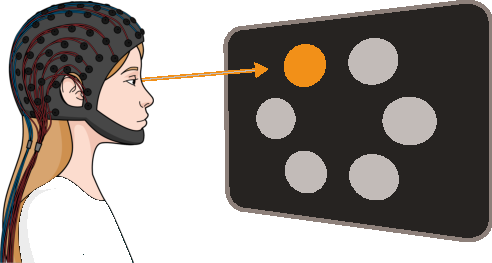
\includegraphics[width=\textwidth]{figures/intro/oddball.pdf}
    %\animategraphics[width=\textwidth]{2}{figures/intro/erp_animation}{}{}
    \smallskip

    \begin{tikzpicture}
      \node at (current page.north east) [%
        anchor=north east,
        text width=7cm,
        fill=white, opacity=1,
        xshift=1cm,
        yshift=-.5cm,
        thin
      ]{%
        \begin{tikzpicture}[trim axis left]
    \begin{axis}[
        width=\textwidth,
        height=0.6180\textwidth,
        xlabel={Time (ms)},
        ylabel={Potential (uV)},
        axis lines=middle,
        ymin=-5, ymax=10,
        xmin=-100, xmax=800,
        ytick={0}, % Y-ticks at -5, 0, 5
        xtick={0}, % X-ticks at 200, 400, 600, 800
      	ylabel near ticks,
      	xlabel near ticks,
    ]

      % Non-target
      \addplot[
          smooth,
          tension=0.5,
          style={very thick,lightgray},
      ] coordinates {%
          (-100, 0)  % Starting point
          (0, 0)     % Baseline
          (50, 0)    % Pre-P1
          (80, 1)    % P1
          (115, -1)  % N1
          (160, 2)   % P2
          (220, -1)   % N2
          (400, 2)   % P3
          (650, 0)   % LPP (Late Positive Potential)
          (800, 0)   % End point
      };


      % Target
      \addplot[
          smooth,
          tension=0.5,
          style={very thick, accent1}, % Set the line color to accent1
      ] coordinates {%
          (-100, 0)  % Starting point
          (0, 0)     % Baseline
          (50, 0)    % Pre-P1
          (80, 2)    % P1
          (115, -3)  % N1
          (160, 3)   % P2
          (220, 1)   % N2
          (400, 7)   % P3
          (650, 1)   % LPP (Late Positive Potential)
          (800, 1)   % End point
      };

      % Annotations for the components
      \small
      \node[anchor=south, color=muteblack] at (axis cs:80,2) {P1};
      \node[anchor=north, color=muteblack] at (axis cs:115,-3) {N1};
      \node[anchor=south, color=muteblack] at (axis cs:160,3) {P2};
      \node[anchor=west, color=muteblack] at (axis cs:220,1) {N2};
      \node[anchor=south, color=muteblack] at (axis cs:400,7) {P3};
      %\node[anchor=south west, color=muteblack] at (axis cs:650,1) {LPP};

    \end{axis}
\end{tikzpicture}%

      };
    \end{tikzpicture}

  \end{minipage}\hfill%
  \begin{minipage}[c]{.5\textwidth}
    \begin{enumerate}
      \item Stimuli flash one by one
      \smallskip
      \item Flashes evoke ERPs
      \smallskip
      \item User attends a stimulus
      \smallskip
      \item ERP components are \\ modulated by attention
      \smallskip
      \item Decode target based on \\ timing and components
    \end{enumerate}
  \end{minipage}
\end{frame}


% =============================================================================

\outline{\emph{C1.} Spatial-temporal ERP decoding}{figures/outline_decode.pdf}
\begin{frame}[c]
  \frametitle{\emph{Problem:} ERP responses can be difficult to extract}
  \begin{minipage}[c]{.5\textwidth}

    Strong noise \ergo machine learning decoders
    \begin{itemize}
      \itemnega High number of features
      \itemnega Calibration: low sample size
    \end{itemize}
    \bigskip

    \emph{Solution}: incorporate original \\ data structure
    \begin{itemize}
      \itemposi Regularization
      \itemposi Fast training
    \end{itemize}
  \end{minipage}\hfill%
  \begin{minipage}[c]{.35\textwidth}
    \centering
    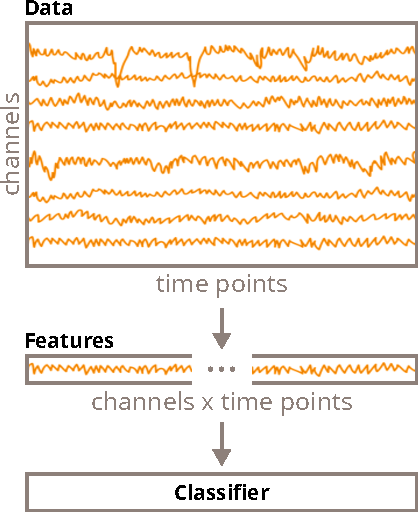
\includegraphics[width=\textwidth]{figures/decode/epoch.pdf}
  \end{minipage}
\end{frame}

\begin{frame}[c]
  \frametitle{Covariance matrix regularization \\
  {\tiny\cite{VanDenKerchove2022}}}
  \begin{minipage}[c]{.3\textwidth}
  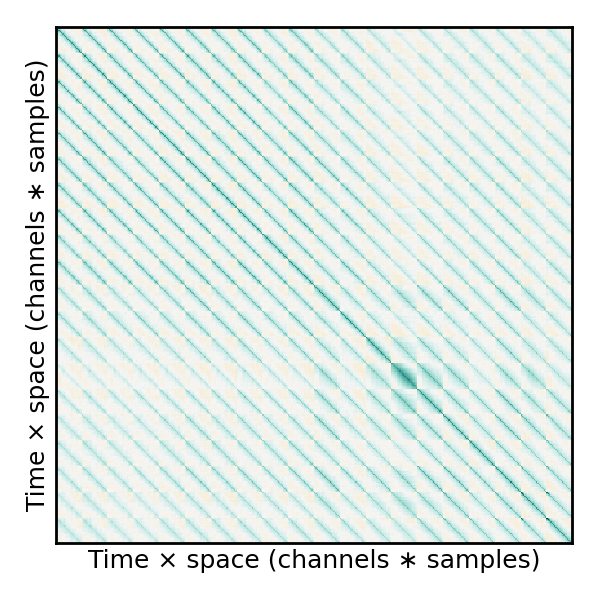
\includegraphics[width=\textwidth]{figures/decode/emp_cov_label.png}
  \end{minipage}
  $=$
  \begin{minipage}[c]{.3\textwidth}
    \begin{minipage}[c]{.4\textwidth}
      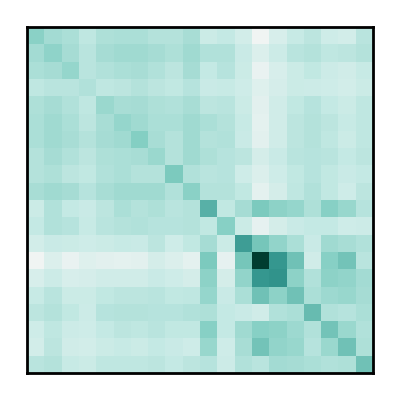
\includegraphics[width=\textwidth]{figures/decode/sp_cov_2.png}
    \end{minipage}
  $\otimes$
    \begin{minipage}[c]{.4\textwidth}
      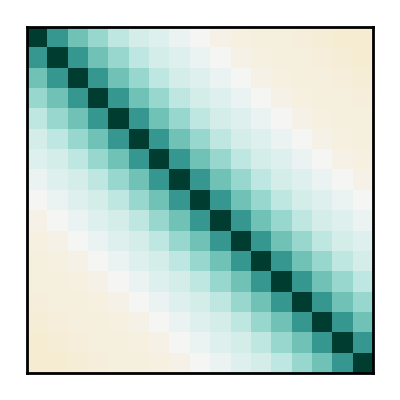
\includegraphics[width=\textwidth]{figures/decode/tmp_cov_2.png}
    \end{minipage}
  \end{minipage}\hfill
  \aside{
    Spatial temporal linear decoders
    \bigskip

    Imprecise due to high number of features
    \bigskip

    Repetitive structure in channels and time
    \bigskip

    Fast computation
    \bigskip

    Improvement for short calibration time

  }


\end{frame}

\begin{frame}
  \frametitle{Spatial-temporal feature extraction}

  \begin{minipage}[t]{.35\linewidth}
		\centering
	%	\begin{tikzpicture}[y=-1cm]
	%		\begin{scope}[shift={(-1,0)}]
  %      \TensorThree{$\ten{X}$}{\rotatebox{90}{\small channels}}{\small time points}{}{2}{2}{0}
	%			\node at (3.2,.5, 2) {$\rightarrow$};
	%			\begin{scope}[shift={(3.25,0.25)}]
	%				\TensorThree{$\ten{G}$}{}{}{}{1}{1}{0}
	%			\end{scope}
	%			\node at (4.2,1.25, 2) {$\downarrow$};
	%			\begin{scope}[shift={(3,2)}]
	%				\TensorTwo{classifier}{}{}{1.5}{.5}
	%			\end{scope}
	%		\end{scope}
  %  \end{tikzpicture}
  %  \bigskip
  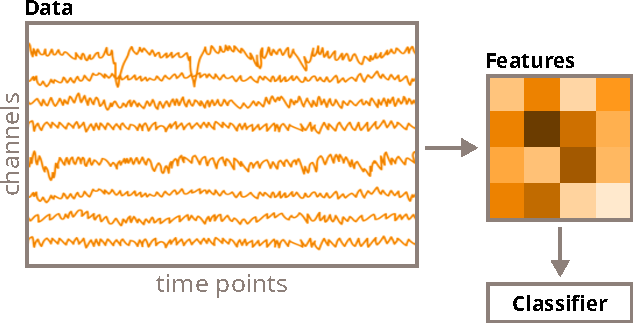
\includegraphics[width=\textwidth]{figures/decode/hoda.pdf}

    \raggedright\small
    Directly operates on structured data
    \begin{itemize}
      \item Extract features separately in space and time
    \end{itemize}
    {\tiny\cite{Phan2010}}
	\end{minipage}\hfill%
  \vrule\hfill%
  \begin{minipage}[t]{.5\textwidth}
    \centering
		%\begin{tikzpicture}[y=-1cm]
		%	\begin{scope}[shift={(-1,0)}]
		%		\TensorThree{$\ten{X}$}{}{}{}{2}{2}{0}
		%		\node at (3.2,.5, 2) {$\rightarrow$};
		%		\begin{scope}[shift={(3.25,0.25)}]
		%			\TensorThree{$\ten{G}^{(1)}$}{}{}{}{1}{1}{0}
		%		\end{scope}
		%		\node at (5.75,.5,2) {$,\cdots,$};
		%		\begin{scope}[shift={(6.25,0.25)}]
		%			\TensorThree{$\ten{G}^{(B)}$}{}{}{}{1}{1}{0}
		%		\end{scope}
		%		\node at (4.2,1.25, 2) {$\downarrow$};
		%		\node at (5.7,1.25, 2) {$\downarrow$};
		%		\node at (7.2,1.25, 2) {$\downarrow$};
		%		\begin{scope}[shift={(3,2)}]
		%			\TensorTwo{classifier}{}{}{4.5}{.5}
		%		\end{scope}
		%	\end{scope}
    %\end{tikzpicture}
    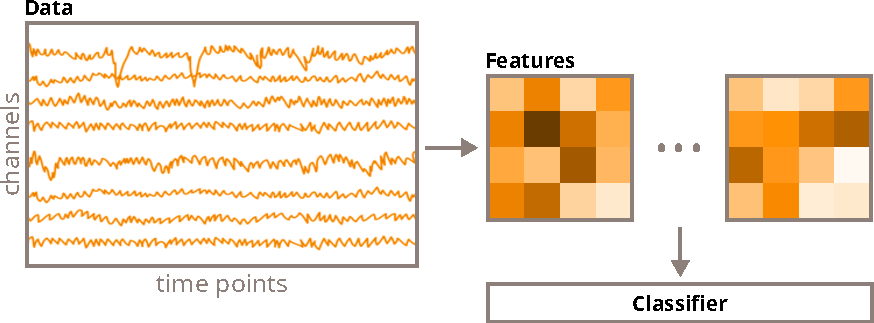
\includegraphics[width=\textwidth]{figures/decode/bttda.pdf}
    \bigskip

    \small
    \begin{minipage}[t]{.45\textwidth}
      \posi\ \ More flexible
      \smallskip

      \posi\ \ Retains structure
      \smallskip

      {\tiny\cite{VanDenKerchovesubmitted}}
    \end{minipage}\hfill%
    \begin{minipage}[t]{.5\textwidth}
      \raggedright
      \nega\ \ More parameters
      \smallskip

      \ergo Heuristic model selection
    \end{minipage}
      \bigskip

      Validated with benchmarking datasets
  \end{minipage}

\end{frame}



% =============================================================================

\outline{\emph{C2.} Eye movement independence}{figures/outline_gaze.pdf}


\begin{frame}
  \frametitle{\emph{Problem:} Eye motor impairment \\  prevents gazing at targets}

  \begin{minipage}[c]{.4\textwidth}
    \raggedright
    Impairment affects BCI operation
    {\tiny\cite{FriedOken2020}}
    {\small
    \begin{itemize}
      \footnotesize
      \item Discomfort fixating
      \item Restricted movement
      \item Involuntary movements
    \end{itemize}
    }
    No direct gaze
    \bigskip
    \bigskip

    Decoding relies on \emph{visual ERP} components \\ {\tiny\cite{Treder2010}}
  \end{minipage}\hfill%
  \begin{minipage}[c]{.55\textwidth}
		\centering
		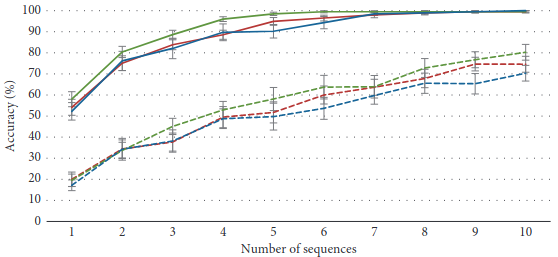
\includegraphics[width=\textwidth]{figures/covert/performance.pdf}

    \raggedleft{\tiny\cite{RonAngevin2019}}


	\end{minipage}
\end{frame}

\begin{frame}
  \frametitle{Covert visuospatial attention experiment \\
    {\tiny\cite{VanDenKerchove2024}}}
    \centering

    \small
    \begin{minipage}{.6\textwidth}
    \begin{minipage}{.3\textwidth}
      overt
      \smallskip

      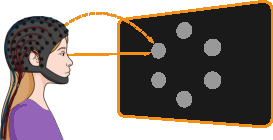
\includegraphics[width=\textwidth]{figures/covert/attention_overt.pdf}
    \end{minipage}\hfill%
    \begin{minipage}{.3\textwidth}
      covert
      \smallskip

      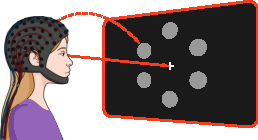
\includegraphics[width=\textwidth]{figures/covert/attention_covert.pdf}
    \end{minipage}\hfill%
    \begin{minipage}{.3\textwidth}
      \small
      split
      \smallskip

      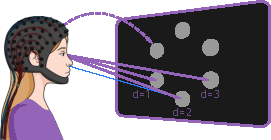
\includegraphics[width=\textwidth]{figures/covert/attention_split.pdf}
    \end{minipage}%
    \end{minipage}
    \bigskip


    \hfill
    \begin{minipage}[c]{.25\textwidth}
    \begin{tikzpicture}[
    scale=\textwidth/5cm
]
% Rectangle background
\fill[muteblack] (-2.5,-2) rectangle (2.5,2);

% Hexagon vertices (white circles)
\fill[white] (1,0) circle (.35);    % Right
\fill[white] (-1,0) circle (.35);   % Left
\fill[white] (0.5,0.866) circle (.35); % Top-right
\fill[white] (-0.5,0.866) circle (.35); % Top-left
\fill[white] (0.5,-0.866) circle (.35); % Bottom-right
\fill[white] (-0.5,-0.866) circle (.35); % Bottom-left
\draw[accent2, ultra thick] (0.9,0) -- (1.1,0);  % Shorter horizontal line
\draw[accent2, ultra thick] (1,-0.1) -- (1,0.1); % Shorter vertical line
\end{tikzpicture}%

      Hex-o-Spell {\tiny\cite{Treder2010}}
    \end{minipage}\hfill%
    \begin{minipage}[c]{.3\textwidth}
      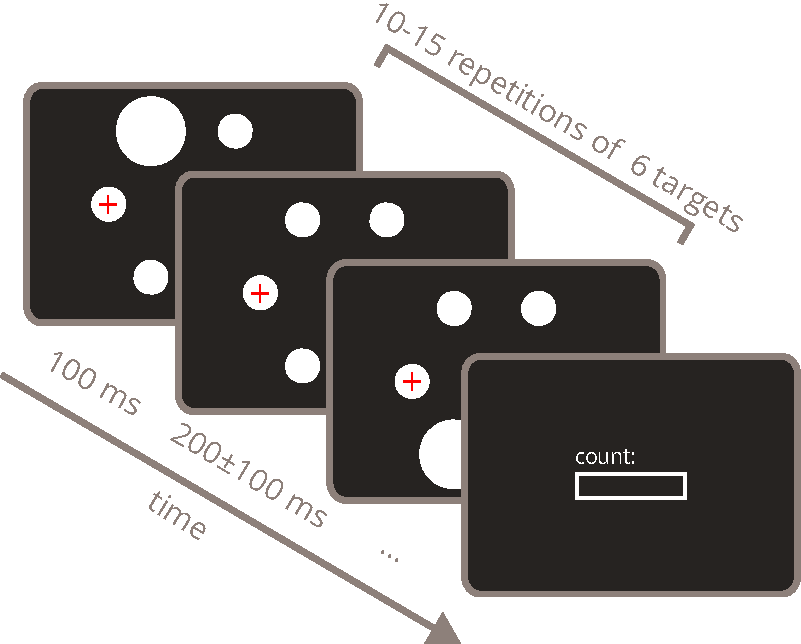
\includegraphics[width=\textwidth]{figures/covert/timeline.pdf}
    \end{minipage}
    \hfill%
    \begin{minipage}[c]{.25\textwidth}
      \begin{itemize}
        \item simulate with 15 healty control subjects
        \item randomized dual attention and gaze task
      \end{itemize}
    \end{minipage}

\end{frame}

\begin{frame}
  \frametitle{Absence of visual ERP components}
  \footnotesize
  \begin{minipage}[t]{.45\textwidth}
    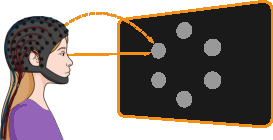
\includegraphics[width=.2\textwidth]{figures/covert/attention_overt.pdf}
    \hspace{.5em}
    \emph{overt}
    \smallskip

    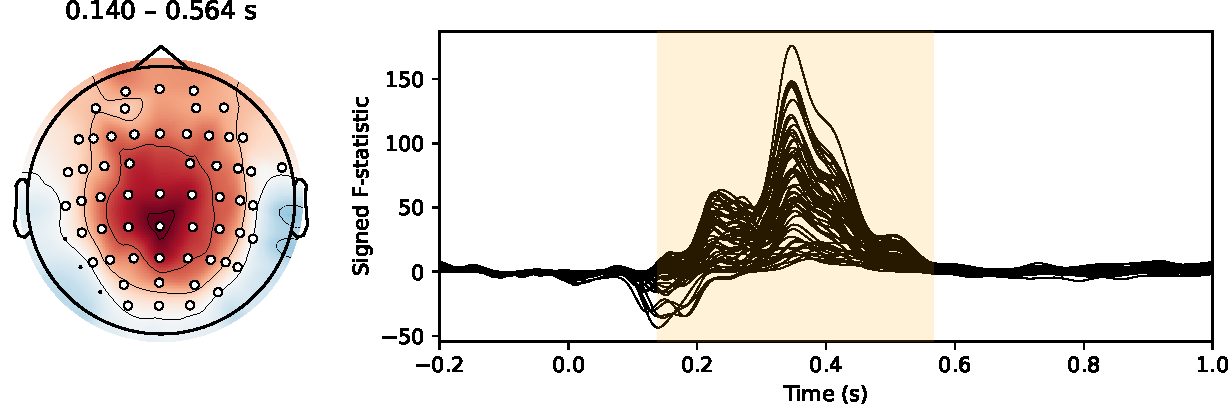
\includegraphics[width=\textwidth]{figures/covert/erps/erp_overt_cluster-1.pdf}
    Attention-based P3 (central-parietal)
    \bigskip

    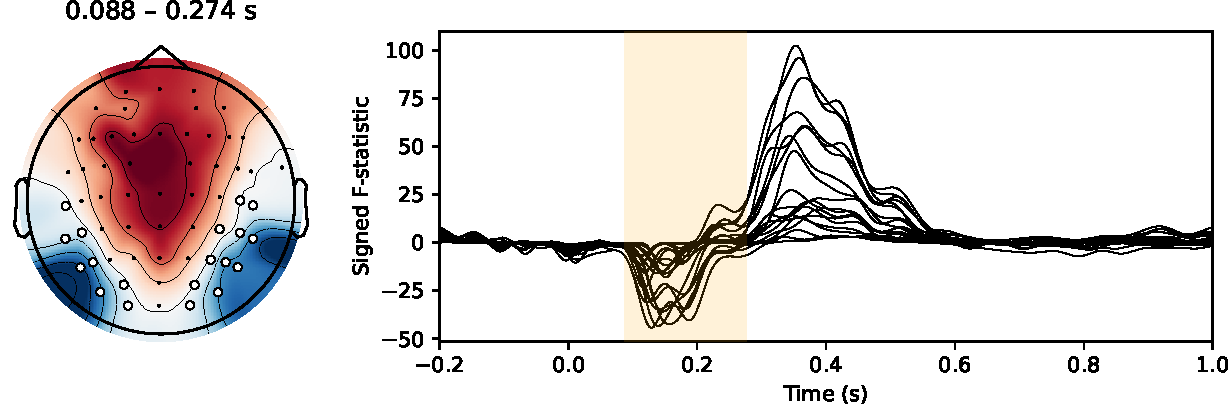
\includegraphics[width=\textwidth]{figures/covert/erps/erp_overt_cluster-0.pdf}
    Visual early components (occipital)
    \smallskip

  \end{minipage}\hfill%
  \begin{minipage}[t]{.45\textwidth}
    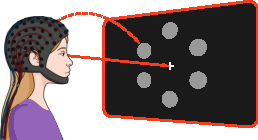
\includegraphics[width=.2\textwidth]{figures/covert/attention_covert.pdf}
    \hspace{.5em}
    \emph{covert}
    \smallskip

    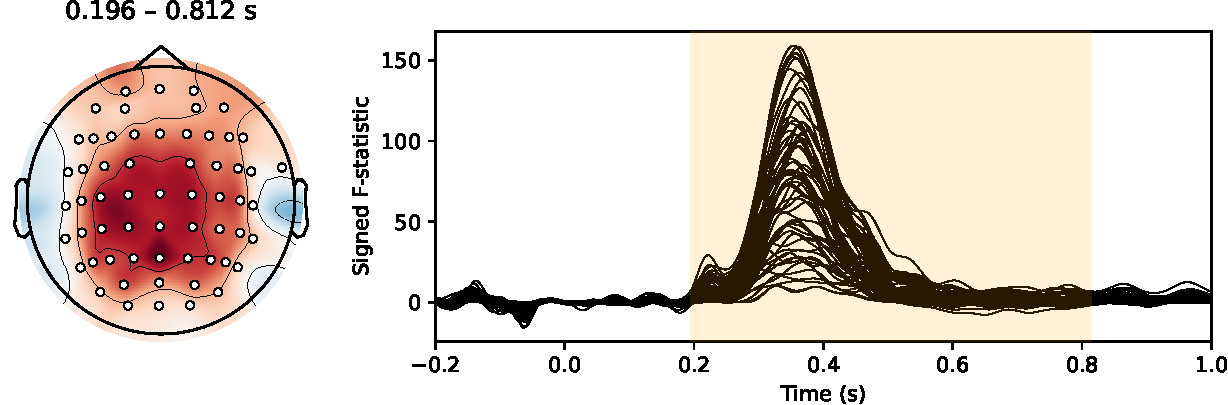
\includegraphics[width=\textwidth]{figures/covert/erps/erp_covert_cluster-0.pdf}
    \smallskip

    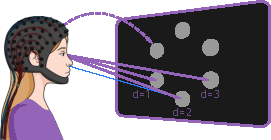
\includegraphics[width=.2\textwidth]{figures/covert/attention_split.pdf}
    \hspace{.5em}
    \emph{split}
    \smallskip

    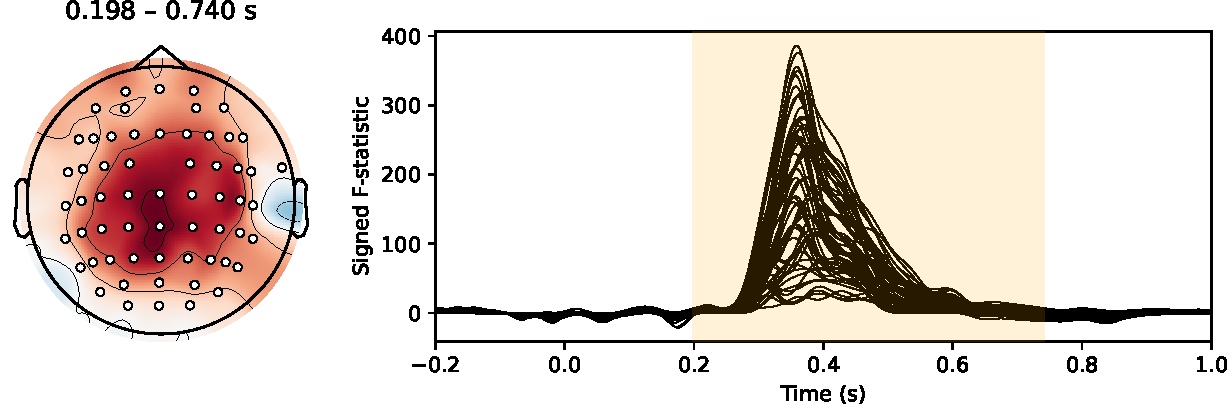
\includegraphics[width=\textwidth]{figures/covert/erps/erp_split_cluster-0.pdf}

  \end{minipage}
  \centering
  \smallskip

  {\tiny F-statistic cluster-based permutation tests}
\end{frame}


%% =============================================================================

\outline{\emph{C3.} Eye movement independent decoding}{figures/outline_decode.pdf}

\begin{frame}[c]
  \frametitle{\emph{Problem:} Latency jitter decreases performance \\ in covert and split
  attention}
  \begin{minipage}{.4\textwidth}
    \centering
\small

\begin{tikzpicture}   % First subplot (low jitter) positioned relative to center
    \begin{axis}[
        at={(0,0)}, % Adjust position to the left, closer to the center
        anchor=center,
        width=\textwidth, height=.7\textwidth,
        xmin=20, xmax=80,
        ymin=-0.1, ymax=1.1,
        axis lines=none, % Remove axes
        title={low jitter}, % Add title
        title style={yshift=-10pt, color=muteblack}, % Adjust title position to make it closer to the plot
        ]
        % Plot individual waveforms (low jitter) in darkgray
        \addplot[darkgray,domain=20:80,samples=100] {exp(-0.5*((x-50)/5)^2)};
        \addplot[darkgray,domain=20:80,samples=100] {exp(-0.5*((x-52)/5)^2)};
        \addplot[darkgray,domain=20:80,samples=100] {exp(-0.5*((x-48)/5)^2)};
        \addplot[darkgray,domain=20:80,samples=100] {exp(-0.5*((x-51)/5)^2)};
        \addplot[darkgray,domain=20:80,samples=100] {exp(-0.5*((x-49)/5)^2)};

        % Plot average waveform (low jitter) in accent1 color, very thick
        \addplot[ultra thick,accent1,domain=20:80,samples=100] {exp(-0.5*((x-50)/5)^2)};
    \end{axis}
\end{tikzpicture}
\bigskip

\begin{tikzpicture}

   % Second subplot (high jitter) positioned relative to center
   \begin{axis}[
      at={(0.55\textwidth,0)}, % Adjust position to the left, closer to the center
       anchor=center,
        width=\textwidth, height=.7\textwidth,
       xmin=20, xmax=80,
       ymin=-0.1, ymax=1.1,
       axis lines=none, % Remove axes
       title={high jitter}, % Add title
       title style={yshift=-10pt, color=muteblack}, % Adjust title position to make it closer to the plot
       ]
       % Plot individual waveforms (high jitter) in darkgray
       \addplot[darkgray,domain=20:80,samples=100] {exp(-0.5*((x-45)/5)^2)};
       \addplot[darkgray,domain=20:80,samples=100] {exp(-0.5*((x-55)/5)^2)};
       \addplot[darkgray,domain=20:80,samples=100] {exp(-0.5*((x-40)/5)^2)};
       \addplot[darkgray,domain=20:80,samples=100] {exp(-0.5*((x-60)/5)^2)};
       \addplot[darkgray,domain=20:80,samples=100] {exp(-0.5*((x-50)/5)^2)};

       % Plot average waveform (high jitter) in accent1 color, very thick
       \addplot[ultra thick,accent1,domain=20:80,samples=100] {0.2*(exp(-0.5*((x-45)/5)^2) + exp(-0.5*((x-55)/5)^2) + exp(-0.5*((x-40)/5)^2) + exp(-0.5*((x-60)/5)^2) + exp(-0.5*((x-50)/5)^2))};
   \end{axis}
\end{tikzpicture}%
\bigskip

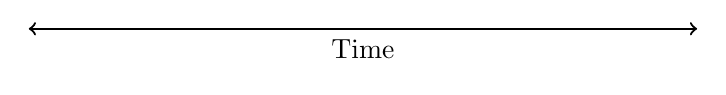
\begin{tikzpicture}
    % Draw the bottom horizontal axis
    \draw[thick,<->] (-0.35\textwidth,-1) -- (.35\textwidth,-1) node[pos=0.5,below] {Time};
\end{tikzpicture}
%\vspace{-5cm}

  \end{minipage}\hfill%
  \begin{minipage}{.55\textwidth}

    \small
    \hspace{3.25em}\emph{CVSA-ERP}\hspace{6.45em}\emph{BNCI2014-009}
    \smallskip

    \centering
    {\centering\resizebox{.7\textwidth}{!}{%
    %CVSA-ERP (our dataset) \hspace{3.5em} BNCI2014-009
    %\smallskip
    \hspace{-0.24572736754045163in}
%%% Creator: Matplotlib, PGF backend
%%
%% To include the figure in your LaTeX document, write
%%   \input{<filename>.pgf}
%%
%% Make sure the required packages are loaded in your preamble
%%   \usepackage{pgf}
%%
%% Also ensure that all the required font packages are loaded; for instance,
%% the lmodern package is sometimes necessary when using math font.
%%   \usepackage{lmodern}
%%
%% Figures using additional raster images can only be included by \input if
%% they are in the same directory as the main LaTeX file. For loading figures
%% from other directories you can use the `import` package
%%   \usepackage{import}
%%
%% and then include the figures with
%%   \import{<path to file>}{<filename>.pgf}
%%
%% Matplotlib used the following preamble
%%   \def\mathdefault#1{#1}
%%   \everymath=\expandafter{\the\everymath\displaystyle}
%%
%%   \ifdefined\pdftexversion\else  % non-pdftex case.
%%     \usepackage{fontspec}
%%   \fi
%%   \makeatletter\@ifpackageloaded{underscore}{}{\usepackage[strings]{underscore}}\makeatother
%%
\begingroup%
\makeatletter%
\begin{pgfpicture}%
\pgfpathrectangle{\pgfpointorigin}{\pgfqpoint{2.997033in}{1.668849in}}%
\pgfusepath{use as bounding box, clip}%
\begin{pgfscope}%
\pgfsetbuttcap%
\pgfsetmiterjoin%
\pgfsetlinewidth{0.000000pt}%
\definecolor{currentstroke}{rgb}{1.000000,1.000000,1.000000}%
\pgfsetstrokecolor{currentstroke}%
\pgfsetstrokeopacity{0.000000}%
\pgfsetdash{}{0pt}%
\pgfpathmoveto{\pgfqpoint{0.000000in}{0.000000in}}%
\pgfpathlineto{\pgfqpoint{2.997033in}{0.000000in}}%
\pgfpathlineto{\pgfqpoint{2.997033in}{1.668849in}}%
\pgfpathlineto{\pgfqpoint{0.000000in}{1.668849in}}%
\pgfpathlineto{\pgfqpoint{0.000000in}{0.000000in}}%
\pgfpathclose%
\pgfusepath{}%
\end{pgfscope}%
\begin{pgfscope}%
\pgfsetbuttcap%
\pgfsetmiterjoin%
\definecolor{currentfill}{rgb}{1.000000,1.000000,1.000000}%
\pgfsetfillcolor{currentfill}%
\pgfsetlinewidth{0.000000pt}%
\definecolor{currentstroke}{rgb}{0.000000,0.000000,0.000000}%
\pgfsetstrokecolor{currentstroke}%
\pgfsetstrokeopacity{0.000000}%
\pgfsetdash{}{0pt}%
\pgfpathmoveto{\pgfqpoint{0.229167in}{0.470139in}}%
\pgfpathlineto{\pgfqpoint{2.146685in}{0.470139in}}%
\pgfpathlineto{\pgfqpoint{2.146685in}{1.608911in}}%
\pgfpathlineto{\pgfqpoint{0.229167in}{1.608911in}}%
\pgfpathlineto{\pgfqpoint{0.229167in}{0.470139in}}%
\pgfpathclose%
\pgfusepath{fill}%
\end{pgfscope}%
\begin{pgfscope}%
\pgfpathrectangle{\pgfqpoint{0.229167in}{0.470139in}}{\pgfqpoint{1.917519in}{1.138772in}}%
\pgfusepath{clip}%
\pgfsetbuttcap%
\pgfsetmiterjoin%
\definecolor{currentfill}{rgb}{0.842157,0.553922,0.200980}%
\pgfsetfillcolor{currentfill}%
\pgfsetlinewidth{0.000000pt}%
\definecolor{currentstroke}{rgb}{0.000000,0.000000,0.000000}%
\pgfsetstrokecolor{currentstroke}%
\pgfsetstrokeopacity{0.000000}%
\pgfsetdash{}{0pt}%
\pgfpathmoveto{\pgfqpoint{0.316327in}{0.470139in}}%
\pgfpathlineto{\pgfqpoint{0.606860in}{0.470139in}}%
\pgfpathlineto{\pgfqpoint{0.606860in}{0.705246in}}%
\pgfpathlineto{\pgfqpoint{0.316327in}{0.705246in}}%
\pgfpathlineto{\pgfqpoint{0.316327in}{0.470139in}}%
\pgfpathclose%
\pgfusepath{fill}%
\end{pgfscope}%
\begin{pgfscope}%
\pgfpathrectangle{\pgfqpoint{0.229167in}{0.470139in}}{\pgfqpoint{1.917519in}{1.138772in}}%
\pgfusepath{clip}%
\pgfsetbuttcap%
\pgfsetmiterjoin%
\definecolor{currentfill}{rgb}{0.858824,0.314706,0.223529}%
\pgfsetfillcolor{currentfill}%
\pgfsetlinewidth{0.000000pt}%
\definecolor{currentstroke}{rgb}{0.000000,0.000000,0.000000}%
\pgfsetstrokecolor{currentstroke}%
\pgfsetstrokeopacity{0.000000}%
\pgfsetdash{}{0pt}%
\pgfpathmoveto{\pgfqpoint{0.679493in}{0.470139in}}%
\pgfpathlineto{\pgfqpoint{0.970026in}{0.470139in}}%
\pgfpathlineto{\pgfqpoint{0.970026in}{1.007696in}}%
\pgfpathlineto{\pgfqpoint{0.679493in}{1.007696in}}%
\pgfpathlineto{\pgfqpoint{0.679493in}{0.470139in}}%
\pgfpathclose%
\pgfusepath{fill}%
\end{pgfscope}%
\begin{pgfscope}%
\pgfpathrectangle{\pgfqpoint{0.229167in}{0.470139in}}{\pgfqpoint{1.917519in}{1.138772in}}%
\pgfusepath{clip}%
\pgfsetbuttcap%
\pgfsetmiterjoin%
\definecolor{currentfill}{rgb}{0.464706,0.320588,0.573529}%
\pgfsetfillcolor{currentfill}%
\pgfsetlinewidth{0.000000pt}%
\definecolor{currentstroke}{rgb}{0.000000,0.000000,0.000000}%
\pgfsetstrokecolor{currentstroke}%
\pgfsetstrokeopacity{0.000000}%
\pgfsetdash{}{0pt}%
\pgfpathmoveto{\pgfqpoint{1.042660in}{0.470139in}}%
\pgfpathlineto{\pgfqpoint{1.333193in}{0.470139in}}%
\pgfpathlineto{\pgfqpoint{1.333193in}{0.979341in}}%
\pgfpathlineto{\pgfqpoint{1.042660in}{0.979341in}}%
\pgfpathlineto{\pgfqpoint{1.042660in}{0.470139in}}%
\pgfpathclose%
\pgfusepath{fill}%
\end{pgfscope}%
\begin{pgfscope}%
\pgfpathrectangle{\pgfqpoint{0.229167in}{0.470139in}}{\pgfqpoint{1.917519in}{1.138772in}}%
\pgfusepath{clip}%
\pgfsetbuttcap%
\pgfsetmiterjoin%
\definecolor{currentfill}{rgb}{0.464706,0.320588,0.573529}%
\pgfsetfillcolor{currentfill}%
\pgfsetlinewidth{0.000000pt}%
\definecolor{currentstroke}{rgb}{0.000000,0.000000,0.000000}%
\pgfsetstrokecolor{currentstroke}%
\pgfsetstrokeopacity{0.000000}%
\pgfsetdash{}{0pt}%
\pgfpathmoveto{\pgfqpoint{1.405826in}{0.470139in}}%
\pgfpathlineto{\pgfqpoint{1.696359in}{0.470139in}}%
\pgfpathlineto{\pgfqpoint{1.696359in}{1.012421in}}%
\pgfpathlineto{\pgfqpoint{1.405826in}{1.012421in}}%
\pgfpathlineto{\pgfqpoint{1.405826in}{0.470139in}}%
\pgfpathclose%
\pgfusepath{fill}%
\end{pgfscope}%
\begin{pgfscope}%
\pgfpathrectangle{\pgfqpoint{0.229167in}{0.470139in}}{\pgfqpoint{1.917519in}{1.138772in}}%
\pgfusepath{clip}%
\pgfsetbuttcap%
\pgfsetmiterjoin%
\definecolor{currentfill}{rgb}{0.464706,0.320588,0.573529}%
\pgfsetfillcolor{currentfill}%
\pgfsetlinewidth{0.000000pt}%
\definecolor{currentstroke}{rgb}{0.000000,0.000000,0.000000}%
\pgfsetstrokecolor{currentstroke}%
\pgfsetstrokeopacity{0.000000}%
\pgfsetdash{}{0pt}%
\pgfpathmoveto{\pgfqpoint{1.768992in}{0.470139in}}%
\pgfpathlineto{\pgfqpoint{2.059526in}{0.470139in}}%
\pgfpathlineto{\pgfqpoint{2.059526in}{0.975797in}}%
\pgfpathlineto{\pgfqpoint{1.768992in}{0.975797in}}%
\pgfpathlineto{\pgfqpoint{1.768992in}{0.470139in}}%
\pgfpathclose%
\pgfusepath{fill}%
\end{pgfscope}%
\begin{pgfscope}%
\pgfsetbuttcap%
\pgfsetroundjoin%
\definecolor{currentfill}{rgb}{0.552941,0.501961,0.478431}%
\pgfsetfillcolor{currentfill}%
\pgfsetlinewidth{0.803000pt}%
\definecolor{currentstroke}{rgb}{0.552941,0.501961,0.478431}%
\pgfsetstrokecolor{currentstroke}%
\pgfsetdash{}{0pt}%
\pgfsys@defobject{currentmarker}{\pgfqpoint{0.000000in}{0.000000in}}{\pgfqpoint{0.000000in}{0.041667in}}{%
\pgfpathmoveto{\pgfqpoint{0.000000in}{0.000000in}}%
\pgfpathlineto{\pgfqpoint{0.000000in}{0.041667in}}%
\pgfusepath{stroke,fill}%
}%
\begin{pgfscope}%
\pgfsys@transformshift{0.461593in}{0.470139in}%
\pgfsys@useobject{currentmarker}{}%
\end{pgfscope}%
\end{pgfscope}%
\begin{pgfscope}%
\definecolor{textcolor}{rgb}{0.552941,0.501961,0.478431}%
\pgfsetstrokecolor{textcolor}%
\pgfsetfillcolor{textcolor}%
\pgftext[x=0.461593in,y=0.421528in,,top]{\color{textcolor}{\sffamily\fontsize{9.000000}{10.800000}\selectfont\catcode`\^=\active\def^{\ifmmode\sp\else\^{}\fi}\catcode`\%=\active\def%{\%}overt}}%
\end{pgfscope}%
\begin{pgfscope}%
\pgfsetbuttcap%
\pgfsetroundjoin%
\definecolor{currentfill}{rgb}{0.552941,0.501961,0.478431}%
\pgfsetfillcolor{currentfill}%
\pgfsetlinewidth{0.803000pt}%
\definecolor{currentstroke}{rgb}{0.552941,0.501961,0.478431}%
\pgfsetstrokecolor{currentstroke}%
\pgfsetdash{}{0pt}%
\pgfsys@defobject{currentmarker}{\pgfqpoint{0.000000in}{0.000000in}}{\pgfqpoint{0.000000in}{0.041667in}}{%
\pgfpathmoveto{\pgfqpoint{0.000000in}{0.000000in}}%
\pgfpathlineto{\pgfqpoint{0.000000in}{0.041667in}}%
\pgfusepath{stroke,fill}%
}%
\begin{pgfscope}%
\pgfsys@transformshift{0.824760in}{0.470139in}%
\pgfsys@useobject{currentmarker}{}%
\end{pgfscope}%
\end{pgfscope}%
\begin{pgfscope}%
\definecolor{textcolor}{rgb}{0.552941,0.501961,0.478431}%
\pgfsetstrokecolor{textcolor}%
\pgfsetfillcolor{textcolor}%
\pgftext[x=0.824760in,y=0.421528in,,top]{\color{textcolor}{\sffamily\fontsize{9.000000}{10.800000}\selectfont\catcode`\^=\active\def^{\ifmmode\sp\else\^{}\fi}\catcode`\%=\active\def%{\%}covert}}%
\end{pgfscope}%
\begin{pgfscope}%
\pgfsetbuttcap%
\pgfsetroundjoin%
\definecolor{currentfill}{rgb}{0.552941,0.501961,0.478431}%
\pgfsetfillcolor{currentfill}%
\pgfsetlinewidth{0.803000pt}%
\definecolor{currentstroke}{rgb}{0.552941,0.501961,0.478431}%
\pgfsetstrokecolor{currentstroke}%
\pgfsetdash{}{0pt}%
\pgfsys@defobject{currentmarker}{\pgfqpoint{0.000000in}{0.000000in}}{\pgfqpoint{0.000000in}{0.041667in}}{%
\pgfpathmoveto{\pgfqpoint{0.000000in}{0.000000in}}%
\pgfpathlineto{\pgfqpoint{0.000000in}{0.041667in}}%
\pgfusepath{stroke,fill}%
}%
\begin{pgfscope}%
\pgfsys@transformshift{1.187926in}{0.470139in}%
\pgfsys@useobject{currentmarker}{}%
\end{pgfscope}%
\end{pgfscope}%
\begin{pgfscope}%
\definecolor{textcolor}{rgb}{0.552941,0.501961,0.478431}%
\pgfsetstrokecolor{textcolor}%
\pgfsetfillcolor{textcolor}%
\pgftext[x=1.076257in, y=0.334722in, left, base]{\color{textcolor}{\sffamily\fontsize{9.000000}{10.800000}\selectfont\catcode`\^=\active\def^{\ifmmode\sp\else\^{}\fi}\catcode`\%=\active\def%{\%}split}}%
\end{pgfscope}%
\begin{pgfscope}%
\definecolor{textcolor}{rgb}{0.552941,0.501961,0.478431}%
\pgfsetstrokecolor{textcolor}%
\pgfsetfillcolor{textcolor}%
\pgftext[x=0.986917in, y=0.197917in, left, base]{\color{textcolor}{\sffamily\fontsize{9.000000}{10.800000}\selectfont\catcode`\^=\active\def^{\ifmmode\sp\else\^{}\fi}\catcode`\%=\active\def%{\%}($d=1$)}}%
\end{pgfscope}%
\begin{pgfscope}%
\pgfsetbuttcap%
\pgfsetroundjoin%
\definecolor{currentfill}{rgb}{0.552941,0.501961,0.478431}%
\pgfsetfillcolor{currentfill}%
\pgfsetlinewidth{0.803000pt}%
\definecolor{currentstroke}{rgb}{0.552941,0.501961,0.478431}%
\pgfsetstrokecolor{currentstroke}%
\pgfsetdash{}{0pt}%
\pgfsys@defobject{currentmarker}{\pgfqpoint{0.000000in}{0.000000in}}{\pgfqpoint{0.000000in}{0.041667in}}{%
\pgfpathmoveto{\pgfqpoint{0.000000in}{0.000000in}}%
\pgfpathlineto{\pgfqpoint{0.000000in}{0.041667in}}%
\pgfusepath{stroke,fill}%
}%
\begin{pgfscope}%
\pgfsys@transformshift{1.551093in}{0.470139in}%
\pgfsys@useobject{currentmarker}{}%
\end{pgfscope}%
\end{pgfscope}%
\begin{pgfscope}%
\definecolor{textcolor}{rgb}{0.552941,0.501961,0.478431}%
\pgfsetstrokecolor{textcolor}%
\pgfsetfillcolor{textcolor}%
\pgftext[x=1.439423in, y=0.334722in, left, base]{\color{textcolor}{\sffamily\fontsize{9.000000}{10.800000}\selectfont\catcode`\^=\active\def^{\ifmmode\sp\else\^{}\fi}\catcode`\%=\active\def%{\%}split}}%
\end{pgfscope}%
\begin{pgfscope}%
\definecolor{textcolor}{rgb}{0.552941,0.501961,0.478431}%
\pgfsetstrokecolor{textcolor}%
\pgfsetfillcolor{textcolor}%
\pgftext[x=1.350083in, y=0.197917in, left, base]{\color{textcolor}{\sffamily\fontsize{9.000000}{10.800000}\selectfont\catcode`\^=\active\def^{\ifmmode\sp\else\^{}\fi}\catcode`\%=\active\def%{\%}($d=2$)}}%
\end{pgfscope}%
\begin{pgfscope}%
\pgfsetbuttcap%
\pgfsetroundjoin%
\definecolor{currentfill}{rgb}{0.552941,0.501961,0.478431}%
\pgfsetfillcolor{currentfill}%
\pgfsetlinewidth{0.803000pt}%
\definecolor{currentstroke}{rgb}{0.552941,0.501961,0.478431}%
\pgfsetstrokecolor{currentstroke}%
\pgfsetdash{}{0pt}%
\pgfsys@defobject{currentmarker}{\pgfqpoint{0.000000in}{0.000000in}}{\pgfqpoint{0.000000in}{0.041667in}}{%
\pgfpathmoveto{\pgfqpoint{0.000000in}{0.000000in}}%
\pgfpathlineto{\pgfqpoint{0.000000in}{0.041667in}}%
\pgfusepath{stroke,fill}%
}%
\begin{pgfscope}%
\pgfsys@transformshift{1.914259in}{0.470139in}%
\pgfsys@useobject{currentmarker}{}%
\end{pgfscope}%
\end{pgfscope}%
\begin{pgfscope}%
\definecolor{textcolor}{rgb}{0.552941,0.501961,0.478431}%
\pgfsetstrokecolor{textcolor}%
\pgfsetfillcolor{textcolor}%
\pgftext[x=1.802590in, y=0.334722in, left, base]{\color{textcolor}{\sffamily\fontsize{9.000000}{10.800000}\selectfont\catcode`\^=\active\def^{\ifmmode\sp\else\^{}\fi}\catcode`\%=\active\def%{\%}split}}%
\end{pgfscope}%
\begin{pgfscope}%
\definecolor{textcolor}{rgb}{0.552941,0.501961,0.478431}%
\pgfsetstrokecolor{textcolor}%
\pgfsetfillcolor{textcolor}%
\pgftext[x=1.713250in, y=0.197917in, left, base]{\color{textcolor}{\sffamily\fontsize{9.000000}{10.800000}\selectfont\catcode`\^=\active\def^{\ifmmode\sp\else\^{}\fi}\catcode`\%=\active\def%{\%}($d=3$)}}%
\end{pgfscope}%
\begin{pgfscope}%
\definecolor{textcolor}{rgb}{0.552941,0.501961,0.478431}%
\pgfsetstrokecolor{textcolor}%
\pgfsetfillcolor{textcolor}%
\pgftext[x=1.187926in,y=0.111111in,,top]{\color{textcolor}{\sffamily\fontsize{9.000000}{10.800000}\selectfont\catcode`\^=\active\def^{\ifmmode\sp\else\^{}\fi}\catcode`\%=\active\def%{\%}VSA condition}}%
\end{pgfscope}%
\begin{pgfscope}%
\pgfsetbuttcap%
\pgfsetroundjoin%
\definecolor{currentfill}{rgb}{0.552941,0.501961,0.478431}%
\pgfsetfillcolor{currentfill}%
\pgfsetlinewidth{0.803000pt}%
\definecolor{currentstroke}{rgb}{0.552941,0.501961,0.478431}%
\pgfsetstrokecolor{currentstroke}%
\pgfsetdash{}{0pt}%
\pgfsys@defobject{currentmarker}{\pgfqpoint{0.000000in}{0.000000in}}{\pgfqpoint{0.041667in}{0.000000in}}{%
\pgfpathmoveto{\pgfqpoint{0.000000in}{0.000000in}}%
\pgfpathlineto{\pgfqpoint{0.041667in}{0.000000in}}%
\pgfusepath{stroke,fill}%
}%
\begin{pgfscope}%
\pgfsys@transformshift{0.229167in}{0.470139in}%
\pgfsys@useobject{currentmarker}{}%
\end{pgfscope}%
\end{pgfscope}%
\begin{pgfscope}%
\pgfsetbuttcap%
\pgfsetroundjoin%
\definecolor{currentfill}{rgb}{0.552941,0.501961,0.478431}%
\pgfsetfillcolor{currentfill}%
\pgfsetlinewidth{0.803000pt}%
\definecolor{currentstroke}{rgb}{0.552941,0.501961,0.478431}%
\pgfsetstrokecolor{currentstroke}%
\pgfsetdash{}{0pt}%
\pgfsys@defobject{currentmarker}{\pgfqpoint{0.000000in}{0.000000in}}{\pgfqpoint{0.041667in}{0.000000in}}{%
\pgfpathmoveto{\pgfqpoint{0.000000in}{0.000000in}}%
\pgfpathlineto{\pgfqpoint{0.041667in}{0.000000in}}%
\pgfusepath{stroke,fill}%
}%
\begin{pgfscope}%
\pgfsys@transformshift{0.229167in}{0.821371in}%
\pgfsys@useobject{currentmarker}{}%
\end{pgfscope}%
\end{pgfscope}%
\begin{pgfscope}%
\pgfsetbuttcap%
\pgfsetroundjoin%
\definecolor{currentfill}{rgb}{0.552941,0.501961,0.478431}%
\pgfsetfillcolor{currentfill}%
\pgfsetlinewidth{0.803000pt}%
\definecolor{currentstroke}{rgb}{0.552941,0.501961,0.478431}%
\pgfsetstrokecolor{currentstroke}%
\pgfsetdash{}{0pt}%
\pgfsys@defobject{currentmarker}{\pgfqpoint{0.000000in}{0.000000in}}{\pgfqpoint{0.041667in}{0.000000in}}{%
\pgfpathmoveto{\pgfqpoint{0.000000in}{0.000000in}}%
\pgfpathlineto{\pgfqpoint{0.041667in}{0.000000in}}%
\pgfusepath{stroke,fill}%
}%
\begin{pgfscope}%
\pgfsys@transformshift{0.229167in}{1.172602in}%
\pgfsys@useobject{currentmarker}{}%
\end{pgfscope}%
\end{pgfscope}%
\begin{pgfscope}%
\pgfsetbuttcap%
\pgfsetroundjoin%
\definecolor{currentfill}{rgb}{0.552941,0.501961,0.478431}%
\pgfsetfillcolor{currentfill}%
\pgfsetlinewidth{0.803000pt}%
\definecolor{currentstroke}{rgb}{0.552941,0.501961,0.478431}%
\pgfsetstrokecolor{currentstroke}%
\pgfsetdash{}{0pt}%
\pgfsys@defobject{currentmarker}{\pgfqpoint{0.000000in}{0.000000in}}{\pgfqpoint{0.041667in}{0.000000in}}{%
\pgfpathmoveto{\pgfqpoint{0.000000in}{0.000000in}}%
\pgfpathlineto{\pgfqpoint{0.041667in}{0.000000in}}%
\pgfusepath{stroke,fill}%
}%
\begin{pgfscope}%
\pgfsys@transformshift{0.229167in}{1.523834in}%
\pgfsys@useobject{currentmarker}{}%
\end{pgfscope}%
\end{pgfscope}%
\begin{pgfscope}%
\definecolor{textcolor}{rgb}{0.552941,0.501961,0.478431}%
\pgfsetstrokecolor{textcolor}%
\pgfsetfillcolor{textcolor}%
\pgftext[x=0.125000in,y=1.039525in,,bottom,rotate=90.000000]{\color{textcolor}{\sffamily\fontsize{9.000000}{10.800000}\selectfont\catcode`\^=\active\def^{\ifmmode\sp\else\^{}\fi}\catcode`\%=\active\def%{\%}Target latency IQR (s)}}%
\end{pgfscope}%
\begin{pgfscope}%
\pgfpathrectangle{\pgfqpoint{0.229167in}{0.470139in}}{\pgfqpoint{1.917519in}{1.138772in}}%
\pgfusepath{clip}%
\pgfsetrectcap%
\pgfsetroundjoin%
\pgfsetlinewidth{2.258437pt}%
\definecolor{currentstroke}{rgb}{0.260000,0.260000,0.260000}%
\pgfsetstrokecolor{currentstroke}%
\pgfsetdash{}{0pt}%
\pgfpathmoveto{\pgfqpoint{0.461593in}{0.635541in}}%
\pgfpathlineto{\pgfqpoint{0.461593in}{0.784403in}}%
\pgfusepath{stroke}%
\end{pgfscope}%
\begin{pgfscope}%
\pgfpathrectangle{\pgfqpoint{0.229167in}{0.470139in}}{\pgfqpoint{1.917519in}{1.138772in}}%
\pgfusepath{clip}%
\pgfsetrectcap%
\pgfsetroundjoin%
\pgfsetlinewidth{2.258437pt}%
\definecolor{currentstroke}{rgb}{0.260000,0.260000,0.260000}%
\pgfsetstrokecolor{currentstroke}%
\pgfsetdash{}{0pt}%
\pgfpathmoveto{\pgfqpoint{0.824760in}{0.978159in}}%
\pgfpathlineto{\pgfqpoint{0.824760in}{1.033687in}}%
\pgfusepath{stroke}%
\end{pgfscope}%
\begin{pgfscope}%
\pgfpathrectangle{\pgfqpoint{0.229167in}{0.470139in}}{\pgfqpoint{1.917519in}{1.138772in}}%
\pgfusepath{clip}%
\pgfsetrectcap%
\pgfsetroundjoin%
\pgfsetlinewidth{2.258437pt}%
\definecolor{currentstroke}{rgb}{0.260000,0.260000,0.260000}%
\pgfsetstrokecolor{currentstroke}%
\pgfsetdash{}{0pt}%
\pgfpathmoveto{\pgfqpoint{1.187926in}{0.928539in}}%
\pgfpathlineto{\pgfqpoint{1.187926in}{1.028961in}}%
\pgfusepath{stroke}%
\end{pgfscope}%
\begin{pgfscope}%
\pgfpathrectangle{\pgfqpoint{0.229167in}{0.470139in}}{\pgfqpoint{1.917519in}{1.138772in}}%
\pgfusepath{clip}%
\pgfsetrectcap%
\pgfsetroundjoin%
\pgfsetlinewidth{2.258437pt}%
\definecolor{currentstroke}{rgb}{0.260000,0.260000,0.260000}%
\pgfsetstrokecolor{currentstroke}%
\pgfsetdash{}{0pt}%
\pgfpathmoveto{\pgfqpoint{1.551093in}{0.954531in}}%
\pgfpathlineto{\pgfqpoint{1.551093in}{1.083308in}}%
\pgfusepath{stroke}%
\end{pgfscope}%
\begin{pgfscope}%
\pgfpathrectangle{\pgfqpoint{0.229167in}{0.470139in}}{\pgfqpoint{1.917519in}{1.138772in}}%
\pgfusepath{clip}%
\pgfsetrectcap%
\pgfsetroundjoin%
\pgfsetlinewidth{2.258437pt}%
\definecolor{currentstroke}{rgb}{0.260000,0.260000,0.260000}%
\pgfsetstrokecolor{currentstroke}%
\pgfsetdash{}{0pt}%
\pgfpathmoveto{\pgfqpoint{1.914259in}{0.940353in}}%
\pgfpathlineto{\pgfqpoint{1.914259in}{1.010088in}}%
\pgfusepath{stroke}%
\end{pgfscope}%
\begin{pgfscope}%
\pgfsetrectcap%
\pgfsetroundjoin%
\pgfsetlinewidth{1.003750pt}%
\definecolor{currentstroke}{rgb}{0.200000,0.200000,0.200000}%
\pgfsetstrokecolor{currentstroke}%
\pgfsetdash{}{0pt}%
\pgfpathmoveto{\pgfqpoint{0.461593in}{1.072317in}}%
\pgfpathlineto{\pgfqpoint{0.461593in}{1.136700in}}%
\pgfpathlineto{\pgfqpoint{0.824760in}{1.136700in}}%
\pgfpathlineto{\pgfqpoint{0.824760in}{1.072317in}}%
\pgfusepath{stroke}%
\end{pgfscope}%
\begin{pgfscope}%
\pgfsetrectcap%
\pgfsetroundjoin%
\pgfsetlinewidth{1.003750pt}%
\definecolor{currentstroke}{rgb}{0.200000,0.200000,0.200000}%
\pgfsetstrokecolor{currentstroke}%
\pgfsetdash{}{0pt}%
\pgfpathmoveto{\pgfqpoint{0.461593in}{1.203918in}}%
\pgfpathlineto{\pgfqpoint{0.461593in}{1.268301in}}%
\pgfpathlineto{\pgfqpoint{1.187926in}{1.268301in}}%
\pgfpathlineto{\pgfqpoint{1.187926in}{1.203918in}}%
\pgfusepath{stroke}%
\end{pgfscope}%
\begin{pgfscope}%
\pgfsetrectcap%
\pgfsetroundjoin%
\pgfsetlinewidth{1.003750pt}%
\definecolor{currentstroke}{rgb}{0.200000,0.200000,0.200000}%
\pgfsetstrokecolor{currentstroke}%
\pgfsetdash{}{0pt}%
\pgfpathmoveto{\pgfqpoint{0.461593in}{1.335519in}}%
\pgfpathlineto{\pgfqpoint{0.461593in}{1.399902in}}%
\pgfpathlineto{\pgfqpoint{1.551093in}{1.399902in}}%
\pgfpathlineto{\pgfqpoint{1.551093in}{1.335519in}}%
\pgfusepath{stroke}%
\end{pgfscope}%
\begin{pgfscope}%
\pgfsetrectcap%
\pgfsetroundjoin%
\pgfsetlinewidth{1.003750pt}%
\definecolor{currentstroke}{rgb}{0.200000,0.200000,0.200000}%
\pgfsetstrokecolor{currentstroke}%
\pgfsetdash{}{0pt}%
\pgfpathmoveto{\pgfqpoint{0.461593in}{1.467120in}}%
\pgfpathlineto{\pgfqpoint{0.461593in}{1.531503in}}%
\pgfpathlineto{\pgfqpoint{1.914259in}{1.531503in}}%
\pgfpathlineto{\pgfqpoint{1.914259in}{1.467120in}}%
\pgfusepath{stroke}%
\end{pgfscope}%
\begin{pgfscope}%
\pgfsetrectcap%
\pgfsetmiterjoin%
\pgfsetlinewidth{0.803000pt}%
\definecolor{currentstroke}{rgb}{0.552941,0.501961,0.478431}%
\pgfsetstrokecolor{currentstroke}%
\pgfsetdash{}{0pt}%
\pgfpathmoveto{\pgfqpoint{0.229167in}{0.470139in}}%
\pgfpathlineto{\pgfqpoint{0.229167in}{1.608911in}}%
\pgfusepath{stroke}%
\end{pgfscope}%
\begin{pgfscope}%
\pgfsetrectcap%
\pgfsetmiterjoin%
\pgfsetlinewidth{0.803000pt}%
\definecolor{currentstroke}{rgb}{0.552941,0.501961,0.478431}%
\pgfsetstrokecolor{currentstroke}%
\pgfsetdash{}{0pt}%
\pgfpathmoveto{\pgfqpoint{0.229167in}{0.470139in}}%
\pgfpathlineto{\pgfqpoint{2.146685in}{0.470139in}}%
\pgfusepath{stroke}%
\end{pgfscope}%
\begin{pgfscope}%
\definecolor{textcolor}{rgb}{0.552941,0.501961,0.478431}%
\pgfsetstrokecolor{textcolor}%
\pgfsetfillcolor{textcolor}%
\pgftext[x=0.643176in,y=1.150589in,,bottom]{\color{textcolor}{\sffamily\fontsize{10.000000}{12.000000}\selectfont\catcode`\^=\active\def^{\ifmmode\sp\else\^{}\fi}\catcode`\%=\active\def%{\%}***}}%
\end{pgfscope}%
\begin{pgfscope}%
\definecolor{textcolor}{rgb}{0.552941,0.501961,0.478431}%
\pgfsetstrokecolor{textcolor}%
\pgfsetfillcolor{textcolor}%
\pgftext[x=0.824760in,y=1.282190in,,bottom]{\color{textcolor}{\sffamily\fontsize{10.000000}{12.000000}\selectfont\catcode`\^=\active\def^{\ifmmode\sp\else\^{}\fi}\catcode`\%=\active\def%{\%}**}}%
\end{pgfscope}%
\begin{pgfscope}%
\definecolor{textcolor}{rgb}{0.552941,0.501961,0.478431}%
\pgfsetstrokecolor{textcolor}%
\pgfsetfillcolor{textcolor}%
\pgftext[x=1.006343in,y=1.413791in,,bottom]{\color{textcolor}{\sffamily\fontsize{10.000000}{12.000000}\selectfont\catcode`\^=\active\def^{\ifmmode\sp\else\^{}\fi}\catcode`\%=\active\def%{\%}**}}%
\end{pgfscope}%
\begin{pgfscope}%
\definecolor{textcolor}{rgb}{0.552941,0.501961,0.478431}%
\pgfsetstrokecolor{textcolor}%
\pgfsetfillcolor{textcolor}%
\pgftext[x=1.187926in,y=1.545392in,,bottom]{\color{textcolor}{\sffamily\fontsize{10.000000}{12.000000}\selectfont\catcode`\^=\active\def^{\ifmmode\sp\else\^{}\fi}\catcode`\%=\active\def%{\%}**}}%
\end{pgfscope}%
\begin{pgfscope}%
\pgfsetbuttcap%
\pgfsetmiterjoin%
\definecolor{currentfill}{rgb}{1.000000,1.000000,1.000000}%
\pgfsetfillcolor{currentfill}%
\pgfsetlinewidth{0.000000pt}%
\definecolor{currentstroke}{rgb}{0.000000,0.000000,0.000000}%
\pgfsetstrokecolor{currentstroke}%
\pgfsetstrokeopacity{0.000000}%
\pgfsetdash{}{0pt}%
\pgfpathmoveto{\pgfqpoint{2.230025in}{0.470139in}}%
\pgfpathlineto{\pgfqpoint{2.997033in}{0.470139in}}%
\pgfpathlineto{\pgfqpoint{2.997033in}{1.608911in}}%
\pgfpathlineto{\pgfqpoint{2.230025in}{1.608911in}}%
\pgfpathlineto{\pgfqpoint{2.230025in}{0.470139in}}%
\pgfpathclose%
\pgfusepath{fill}%
\end{pgfscope}%
\begin{pgfscope}%
\pgfpathrectangle{\pgfqpoint{2.230025in}{0.470139in}}{\pgfqpoint{0.767008in}{1.138772in}}%
\pgfusepath{clip}%
\pgfsetbuttcap%
\pgfsetmiterjoin%
\definecolor{currentfill}{rgb}{0.842157,0.553922,0.200980}%
\pgfsetfillcolor{currentfill}%
\pgfsetlinewidth{0.000000pt}%
\definecolor{currentstroke}{rgb}{0.000000,0.000000,0.000000}%
\pgfsetstrokecolor{currentstroke}%
\pgfsetstrokeopacity{0.000000}%
\pgfsetdash{}{0pt}%
\pgfpathmoveto{\pgfqpoint{2.264889in}{0.470139in}}%
\pgfpathlineto{\pgfqpoint{2.574792in}{0.470139in}}%
\pgfpathlineto{\pgfqpoint{2.574792in}{0.693995in}}%
\pgfpathlineto{\pgfqpoint{2.264889in}{0.693995in}}%
\pgfpathlineto{\pgfqpoint{2.264889in}{0.470139in}}%
\pgfpathclose%
\pgfusepath{fill}%
\end{pgfscope}%
\begin{pgfscope}%
\pgfpathrectangle{\pgfqpoint{2.230025in}{0.470139in}}{\pgfqpoint{0.767008in}{1.138772in}}%
\pgfusepath{clip}%
\pgfsetbuttcap%
\pgfsetmiterjoin%
\definecolor{currentfill}{rgb}{0.858824,0.314706,0.223529}%
\pgfsetfillcolor{currentfill}%
\pgfsetlinewidth{0.000000pt}%
\definecolor{currentstroke}{rgb}{0.000000,0.000000,0.000000}%
\pgfsetstrokecolor{currentstroke}%
\pgfsetstrokeopacity{0.000000}%
\pgfsetdash{}{0pt}%
\pgfpathmoveto{\pgfqpoint{2.652267in}{0.470139in}}%
\pgfpathlineto{\pgfqpoint{2.962169in}{0.470139in}}%
\pgfpathlineto{\pgfqpoint{2.962169in}{0.862361in}}%
\pgfpathlineto{\pgfqpoint{2.652267in}{0.862361in}}%
\pgfpathlineto{\pgfqpoint{2.652267in}{0.470139in}}%
\pgfpathclose%
\pgfusepath{fill}%
\end{pgfscope}%
\begin{pgfscope}%
\pgfsetbuttcap%
\pgfsetroundjoin%
\definecolor{currentfill}{rgb}{0.552941,0.501961,0.478431}%
\pgfsetfillcolor{currentfill}%
\pgfsetlinewidth{0.803000pt}%
\definecolor{currentstroke}{rgb}{0.552941,0.501961,0.478431}%
\pgfsetstrokecolor{currentstroke}%
\pgfsetdash{}{0pt}%
\pgfsys@defobject{currentmarker}{\pgfqpoint{0.000000in}{0.000000in}}{\pgfqpoint{0.000000in}{0.041667in}}{%
\pgfpathmoveto{\pgfqpoint{0.000000in}{0.000000in}}%
\pgfpathlineto{\pgfqpoint{0.000000in}{0.041667in}}%
\pgfusepath{stroke,fill}%
}%
\begin{pgfscope}%
\pgfsys@transformshift{2.419840in}{0.470139in}%
\pgfsys@useobject{currentmarker}{}%
\end{pgfscope}%
\end{pgfscope}%
\begin{pgfscope}%
\definecolor{textcolor}{rgb}{0.552941,0.501961,0.478431}%
\pgfsetstrokecolor{textcolor}%
\pgfsetfillcolor{textcolor}%
\pgftext[x=2.419840in,y=0.421528in,,top]{\color{textcolor}{\sffamily\fontsize{9.000000}{10.800000}\selectfont\catcode`\^=\active\def^{\ifmmode\sp\else\^{}\fi}\catcode`\%=\active\def%{\%}overt}}%
\end{pgfscope}%
\begin{pgfscope}%
\pgfsetbuttcap%
\pgfsetroundjoin%
\definecolor{currentfill}{rgb}{0.552941,0.501961,0.478431}%
\pgfsetfillcolor{currentfill}%
\pgfsetlinewidth{0.803000pt}%
\definecolor{currentstroke}{rgb}{0.552941,0.501961,0.478431}%
\pgfsetstrokecolor{currentstroke}%
\pgfsetdash{}{0pt}%
\pgfsys@defobject{currentmarker}{\pgfqpoint{0.000000in}{0.000000in}}{\pgfqpoint{0.000000in}{0.041667in}}{%
\pgfpathmoveto{\pgfqpoint{0.000000in}{0.000000in}}%
\pgfpathlineto{\pgfqpoint{0.000000in}{0.041667in}}%
\pgfusepath{stroke,fill}%
}%
\begin{pgfscope}%
\pgfsys@transformshift{2.807218in}{0.470139in}%
\pgfsys@useobject{currentmarker}{}%
\end{pgfscope}%
\end{pgfscope}%
\begin{pgfscope}%
\definecolor{textcolor}{rgb}{0.552941,0.501961,0.478431}%
\pgfsetstrokecolor{textcolor}%
\pgfsetfillcolor{textcolor}%
\pgftext[x=2.807218in,y=0.421528in,,top]{\color{textcolor}{\sffamily\fontsize{9.000000}{10.800000}\selectfont\catcode`\^=\active\def^{\ifmmode\sp\else\^{}\fi}\catcode`\%=\active\def%{\%}covert}}%
\end{pgfscope}%
\begin{pgfscope}%
\definecolor{textcolor}{rgb}{0.552941,0.501961,0.478431}%
\pgfsetstrokecolor{textcolor}%
\pgfsetfillcolor{textcolor}%
\pgftext[x=2.613529in,y=0.254861in,,top]{\color{textcolor}{\sffamily\fontsize{9.000000}{10.800000}\selectfont\catcode`\^=\active\def^{\ifmmode\sp\else\^{}\fi}\catcode`\%=\active\def%{\%}VSA condition}}%
\end{pgfscope}%
\begin{pgfscope}%
\pgfsetbuttcap%
\pgfsetroundjoin%
\definecolor{currentfill}{rgb}{0.552941,0.501961,0.478431}%
\pgfsetfillcolor{currentfill}%
\pgfsetlinewidth{0.803000pt}%
\definecolor{currentstroke}{rgb}{0.552941,0.501961,0.478431}%
\pgfsetstrokecolor{currentstroke}%
\pgfsetdash{}{0pt}%
\pgfsys@defobject{currentmarker}{\pgfqpoint{0.000000in}{0.000000in}}{\pgfqpoint{0.041667in}{0.000000in}}{%
\pgfpathmoveto{\pgfqpoint{0.000000in}{0.000000in}}%
\pgfpathlineto{\pgfqpoint{0.041667in}{0.000000in}}%
\pgfusepath{stroke,fill}%
}%
\begin{pgfscope}%
\pgfsys@transformshift{2.230025in}{0.470139in}%
\pgfsys@useobject{currentmarker}{}%
\end{pgfscope}%
\end{pgfscope}%
\begin{pgfscope}%
\pgfsetbuttcap%
\pgfsetroundjoin%
\definecolor{currentfill}{rgb}{0.552941,0.501961,0.478431}%
\pgfsetfillcolor{currentfill}%
\pgfsetlinewidth{0.803000pt}%
\definecolor{currentstroke}{rgb}{0.552941,0.501961,0.478431}%
\pgfsetstrokecolor{currentstroke}%
\pgfsetdash{}{0pt}%
\pgfsys@defobject{currentmarker}{\pgfqpoint{0.000000in}{0.000000in}}{\pgfqpoint{0.041667in}{0.000000in}}{%
\pgfpathmoveto{\pgfqpoint{0.000000in}{0.000000in}}%
\pgfpathlineto{\pgfqpoint{0.041667in}{0.000000in}}%
\pgfusepath{stroke,fill}%
}%
\begin{pgfscope}%
\pgfsys@transformshift{2.230025in}{0.821371in}%
\pgfsys@useobject{currentmarker}{}%
\end{pgfscope}%
\end{pgfscope}%
\begin{pgfscope}%
\pgfsetbuttcap%
\pgfsetroundjoin%
\definecolor{currentfill}{rgb}{0.552941,0.501961,0.478431}%
\pgfsetfillcolor{currentfill}%
\pgfsetlinewidth{0.803000pt}%
\definecolor{currentstroke}{rgb}{0.552941,0.501961,0.478431}%
\pgfsetstrokecolor{currentstroke}%
\pgfsetdash{}{0pt}%
\pgfsys@defobject{currentmarker}{\pgfqpoint{0.000000in}{0.000000in}}{\pgfqpoint{0.041667in}{0.000000in}}{%
\pgfpathmoveto{\pgfqpoint{0.000000in}{0.000000in}}%
\pgfpathlineto{\pgfqpoint{0.041667in}{0.000000in}}%
\pgfusepath{stroke,fill}%
}%
\begin{pgfscope}%
\pgfsys@transformshift{2.230025in}{1.172602in}%
\pgfsys@useobject{currentmarker}{}%
\end{pgfscope}%
\end{pgfscope}%
\begin{pgfscope}%
\pgfsetbuttcap%
\pgfsetroundjoin%
\definecolor{currentfill}{rgb}{0.552941,0.501961,0.478431}%
\pgfsetfillcolor{currentfill}%
\pgfsetlinewidth{0.803000pt}%
\definecolor{currentstroke}{rgb}{0.552941,0.501961,0.478431}%
\pgfsetstrokecolor{currentstroke}%
\pgfsetdash{}{0pt}%
\pgfsys@defobject{currentmarker}{\pgfqpoint{0.000000in}{0.000000in}}{\pgfqpoint{0.041667in}{0.000000in}}{%
\pgfpathmoveto{\pgfqpoint{0.000000in}{0.000000in}}%
\pgfpathlineto{\pgfqpoint{0.041667in}{0.000000in}}%
\pgfusepath{stroke,fill}%
}%
\begin{pgfscope}%
\pgfsys@transformshift{2.230025in}{1.523834in}%
\pgfsys@useobject{currentmarker}{}%
\end{pgfscope}%
\end{pgfscope}%
\begin{pgfscope}%
\pgfpathrectangle{\pgfqpoint{2.230025in}{0.470139in}}{\pgfqpoint{0.767008in}{1.138772in}}%
\pgfusepath{clip}%
\pgfsetrectcap%
\pgfsetroundjoin%
\pgfsetlinewidth{2.258437pt}%
\definecolor{currentstroke}{rgb}{0.260000,0.260000,0.260000}%
\pgfsetstrokecolor{currentstroke}%
\pgfsetdash{}{0pt}%
\pgfpathmoveto{\pgfqpoint{2.419840in}{0.661733in}}%
\pgfpathlineto{\pgfqpoint{2.419840in}{0.729103in}}%
\pgfusepath{stroke}%
\end{pgfscope}%
\begin{pgfscope}%
\pgfpathrectangle{\pgfqpoint{2.230025in}{0.470139in}}{\pgfqpoint{0.767008in}{1.138772in}}%
\pgfusepath{clip}%
\pgfsetrectcap%
\pgfsetroundjoin%
\pgfsetlinewidth{2.258437pt}%
\definecolor{currentstroke}{rgb}{0.260000,0.260000,0.260000}%
\pgfsetstrokecolor{currentstroke}%
\pgfsetdash{}{0pt}%
\pgfpathmoveto{\pgfqpoint{2.807218in}{0.829162in}}%
\pgfpathlineto{\pgfqpoint{2.807218in}{0.901263in}}%
\pgfusepath{stroke}%
\end{pgfscope}%
\begin{pgfscope}%
\pgfsetrectcap%
\pgfsetroundjoin%
\pgfsetlinewidth{1.003750pt}%
\definecolor{currentstroke}{rgb}{0.200000,0.200000,0.200000}%
\pgfsetstrokecolor{currentstroke}%
\pgfsetdash{}{0pt}%
\pgfpathmoveto{\pgfqpoint{2.419840in}{0.969590in}}%
\pgfpathlineto{\pgfqpoint{2.419840in}{1.083467in}}%
\pgfpathlineto{\pgfqpoint{2.807218in}{1.083467in}}%
\pgfpathlineto{\pgfqpoint{2.807218in}{0.969590in}}%
\pgfusepath{stroke}%
\end{pgfscope}%
\begin{pgfscope}%
\pgfsetrectcap%
\pgfsetmiterjoin%
\pgfsetlinewidth{0.803000pt}%
\definecolor{currentstroke}{rgb}{0.552941,0.501961,0.478431}%
\pgfsetstrokecolor{currentstroke}%
\pgfsetdash{}{0pt}%
\pgfpathmoveto{\pgfqpoint{2.230025in}{0.470139in}}%
\pgfpathlineto{\pgfqpoint{2.230025in}{1.608911in}}%
\pgfusepath{stroke}%
\end{pgfscope}%
\begin{pgfscope}%
\pgfsetrectcap%
\pgfsetmiterjoin%
\pgfsetlinewidth{0.803000pt}%
\definecolor{currentstroke}{rgb}{0.552941,0.501961,0.478431}%
\pgfsetstrokecolor{currentstroke}%
\pgfsetdash{}{0pt}%
\pgfpathmoveto{\pgfqpoint{2.230025in}{0.470139in}}%
\pgfpathlineto{\pgfqpoint{2.997033in}{0.470139in}}%
\pgfusepath{stroke}%
\end{pgfscope}%
\begin{pgfscope}%
\definecolor{textcolor}{rgb}{0.552941,0.501961,0.478431}%
\pgfsetstrokecolor{textcolor}%
\pgfsetfillcolor{textcolor}%
\pgftext[x=2.613529in,y=1.097356in,,bottom]{\color{textcolor}{\sffamily\fontsize{10.000000}{12.000000}\selectfont\catcode`\^=\active\def^{\ifmmode\sp\else\^{}\fi}\catcode`\%=\active\def%{\%}****}}%
\end{pgfscope}%
\end{pgfpicture}%
\makeatother%
\endgroup%

    }}

    \begin{itemize}
      %\item Classifier-based latency estimation {\tiny\cite{Mowla2017}}
      \item Higher jitter when eye movement independent
      \item Contributes to low accuracy \\ {\tiny\cite{Arico2014}}
      \item Can this be \emph{accounted for}?
    \end{itemize}

  \end{minipage}

\end{frame}

\begin{frame}
  \frametitle{Latency estimation and alignment}
  \begin{minipage}{.3\textwidth}
    \centering
    \emph{Before} alignment
    \smallskip

    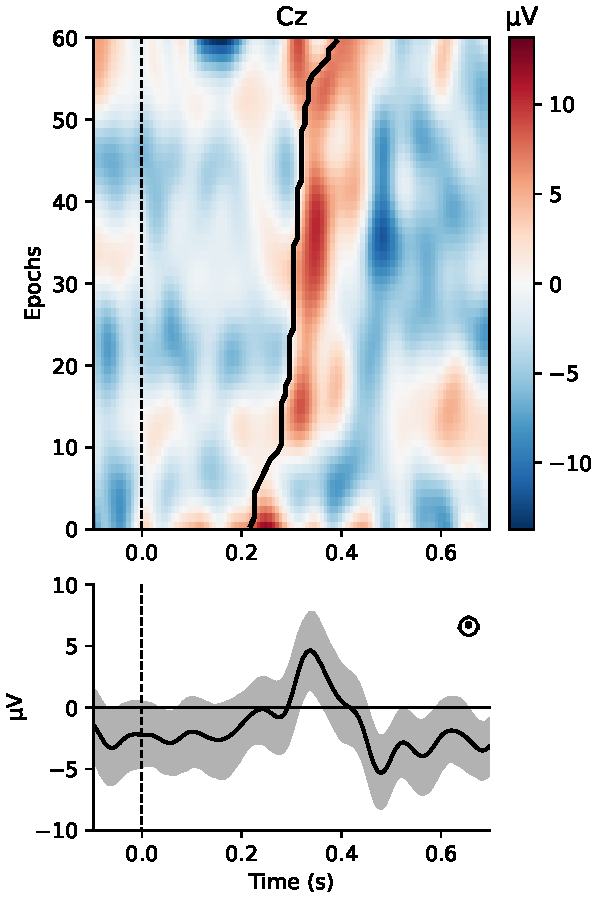
\includegraphics[width=\textwidth]{figures/covert/align_before.pdf}
  \end{minipage}
  \begin{minipage}{.3\textwidth}
    \centering
    \emph{After} alignment
    \smallskip

    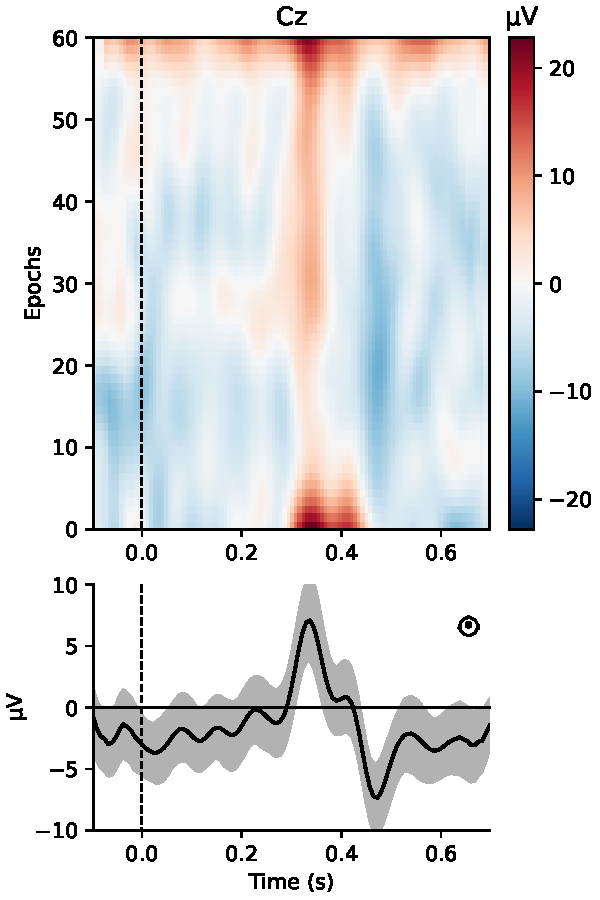
\includegraphics[width=\textwidth]{figures/covert/align_after.pdf}
  \end{minipage}
  \aside{%
    Developed enhanced ERP latency estimation method
    {\tiny\cite{VanDenKerchove2024,Mowla2017}}
    \bigskip

    Iterative alignment
    \bigskip

    Improves latency estimation in simulated data
    \bigskip

    Useful in BCI setting?
  }
\end{frame}


\begin{frame}
  \frametitle{Application to eye movement independent \\ decoding}
  \begin{minipage}{.6\textwidth}
    \centering
    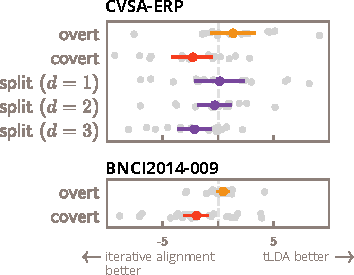
\includegraphics[width=\textwidth]{figures/covert/roc_auc_diff.pdf}
  \end{minipage}\hfill
  \aside{%
    Applicable as decoder
    \bigskip

    Within-subject, cross-validated ROC-AUC
    \bigskip

    Compared with state-\\of-the art decoder (tLDA) \\
    {\tiny\cite{Sosulski2022}}
    \bigskip

    Improves decoding performance if no gaze


  }
\end{frame}

% =============================================================================

\outline{\emph{C4:} Evaluation in end-users}{figures/outline_patient.pdf}

\begin{frame}
  \frametitle{Participants with physical, speech and eye movement
  impairment}

    \hfill
    \begin{minipage}[t]{.3\textwidth}
      3 Friedreich's \emph{ataxia}
       \begin{itemize}
          \item impaired speech
          \item involuntary eye movements
          \item discomfort fixating
        \end{itemize}
    \end{minipage}\hfill%
    \begin{minipage}[t]{.3\textwidth}
      1 bulbar onset \emph{ALS}
       \begin{itemize}
          \item no speech
          \item minor eye movement impairment
        \end{itemize}
    \end{minipage}\hfill%
    \begin{minipage}[t]{.3\textwidth}
      3 brain stem or cerebellar \emph{stroke}
       \begin{itemize}
          \item no speech
          \item partial eye paralysis
       \end{itemize}
    \end{minipage}
    \hfill
    \bigskip
    \bigskip

    \centering
    Large \emph{individual variety} in preserved skills
    \bigskip
    \bigskip

    \hfill
    
\includegraphics[height=.075\textwidth]{figures/logos/uz_leuven.jpg}
    \hfill
    
\includegraphics[height=.1\textwidth]{figures/logos/chu_lille.png}
    \hfill
    
\includegraphics[height=.05\textwidth]{figures/logos/trainm.png}
    \hfill
    
\includegraphics[height=.1\textwidth]{figures/logos/fondation-partage-vie.png}
    \hfill
\end{frame}

\begin{frame}
  \frametitle{Covert visuospatial attention experiment}

  \begin{minipage}{.6\textwidth}
    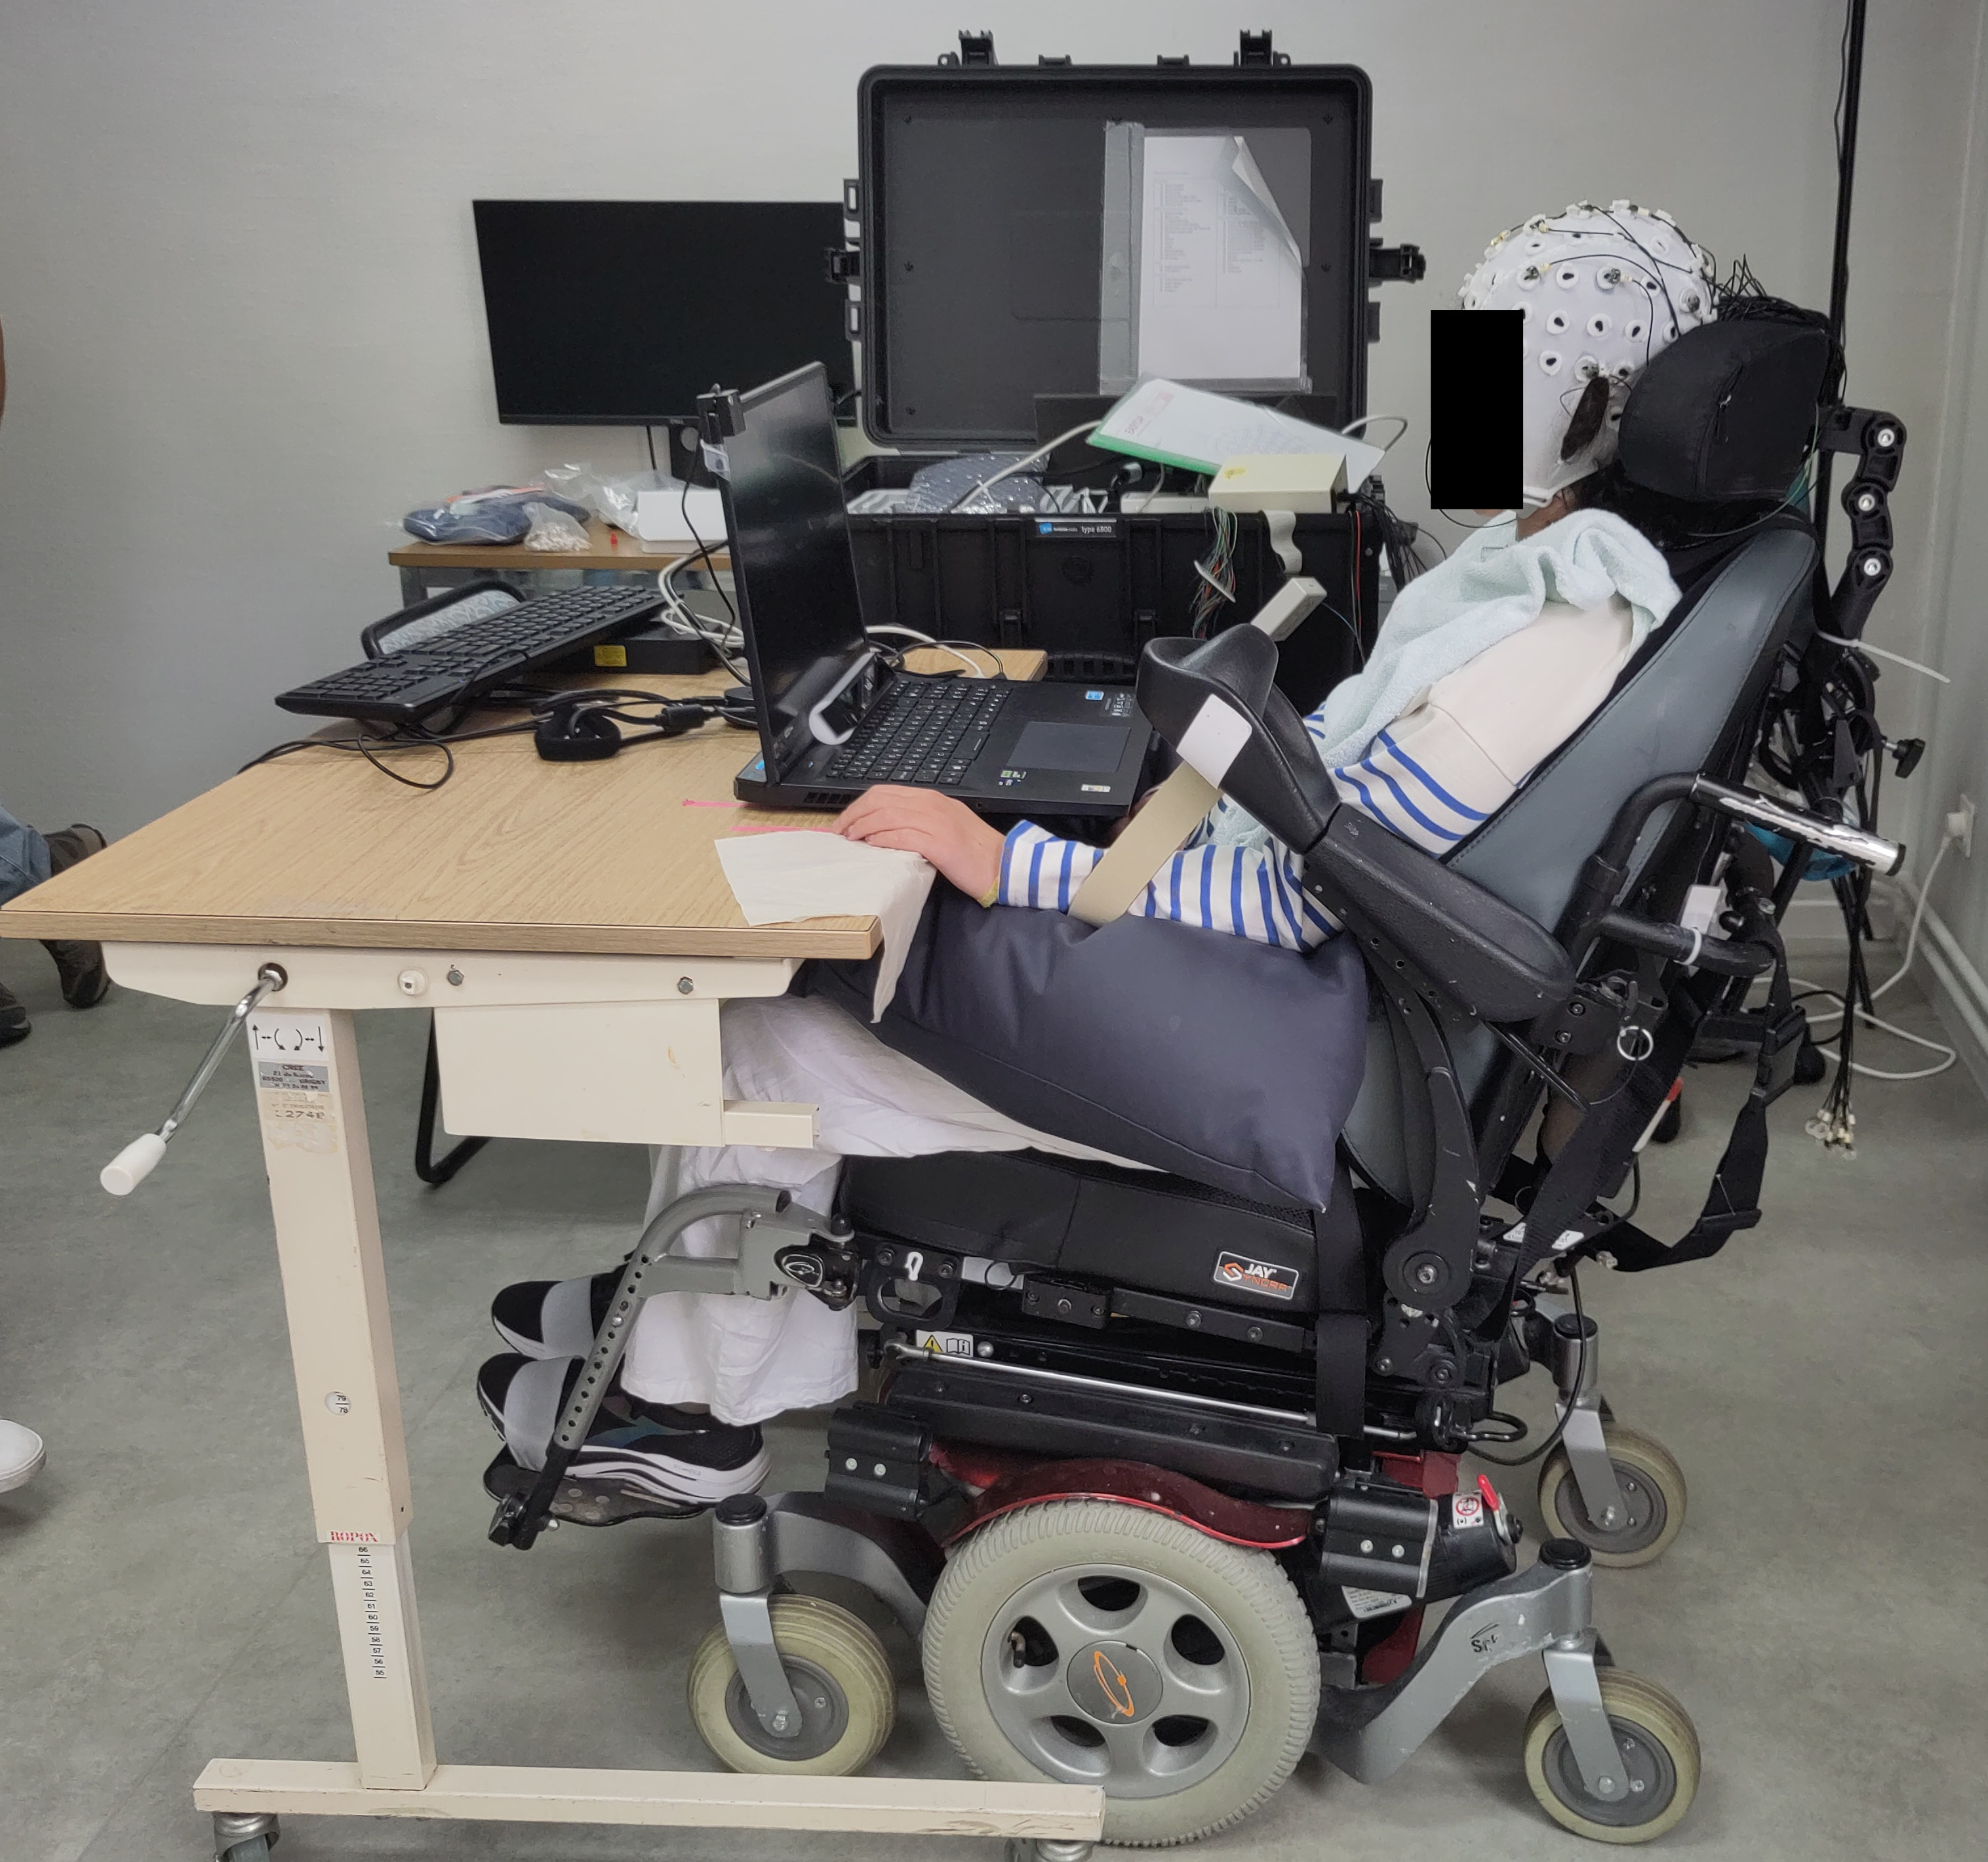
\includegraphics[height=.45\textwidth]{figures/patients/PD01a-obfuscated.jpg}%
    \hfill%
    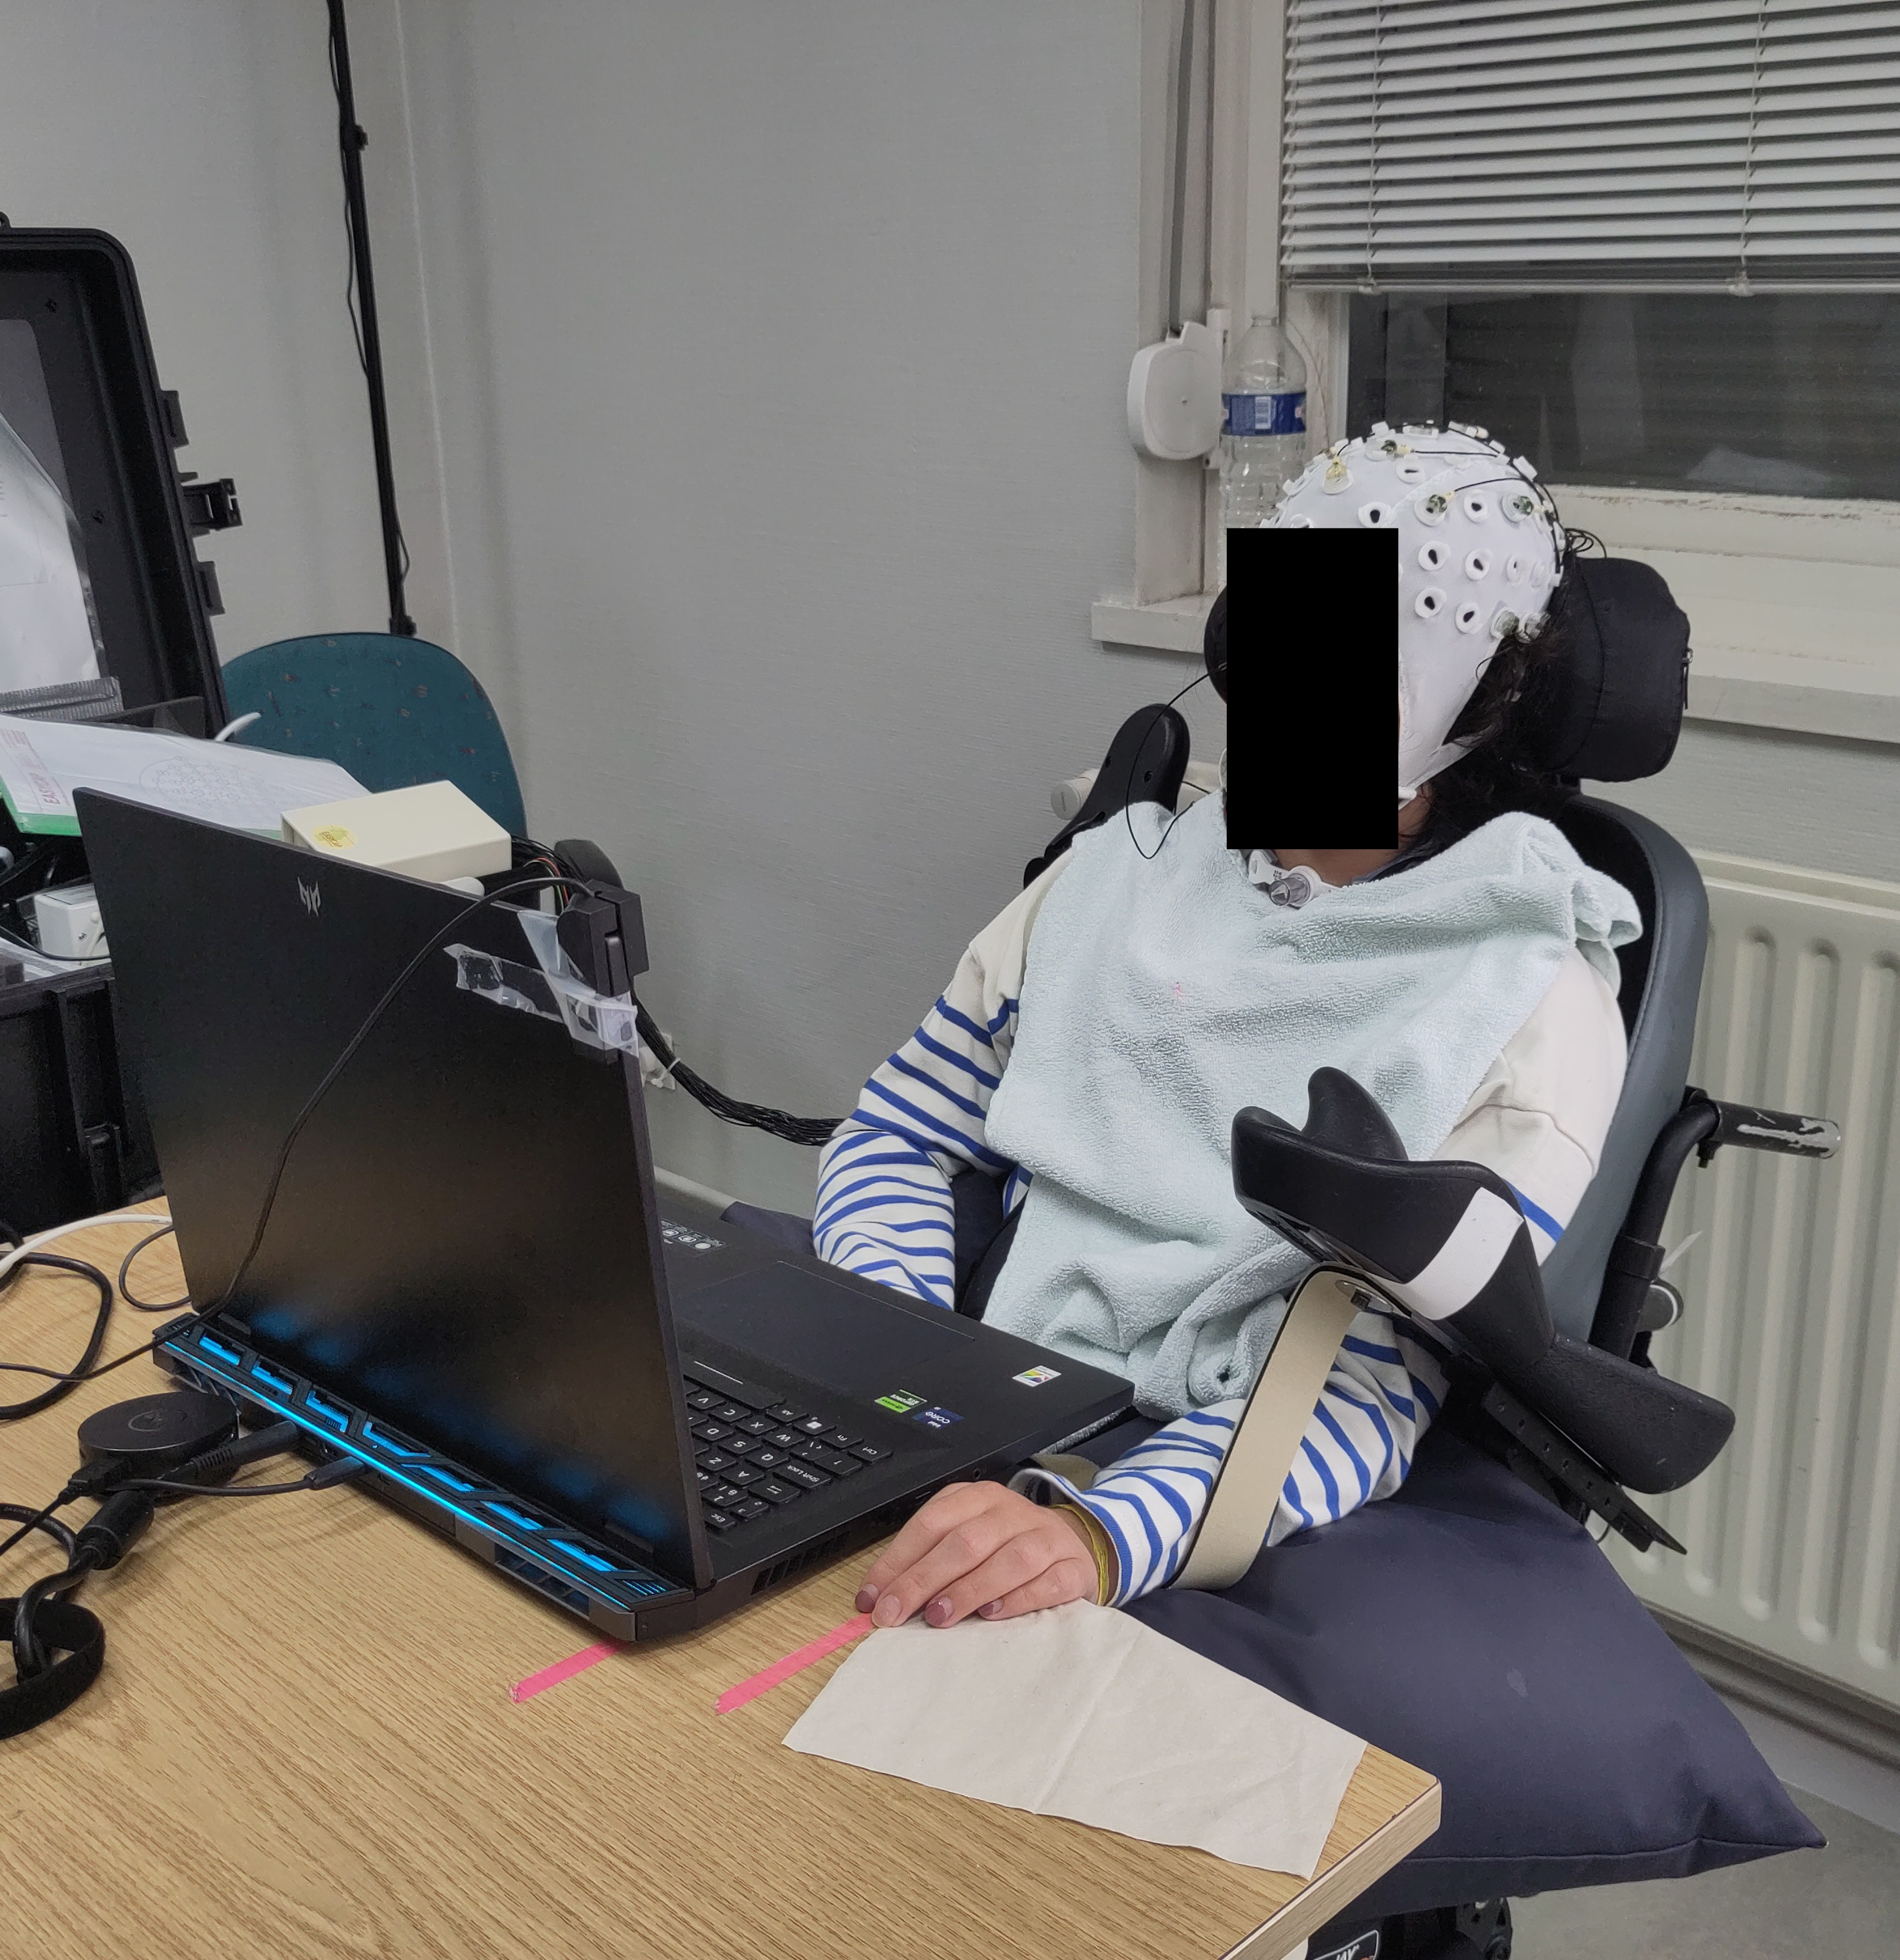
\includegraphics[height=.45\textwidth]{figures/patients/PD01b-obfuscated.jpg}%
    \bigskip

    {\small
    \begin{minipage}{.3\textwidth}
      overt
      \smallskip

      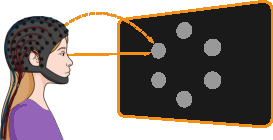
\includegraphics[width=\textwidth]{figures/covert/attention_overt.pdf}
    \end{minipage}\hfill%
    \begin{minipage}{.3\textwidth}
      covert
      \smallskip

      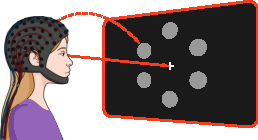
\includegraphics[width=\textwidth]{figures/covert/attention_covert.pdf}
    \end{minipage}\hfill%
    \begin{minipage}{.3\textwidth}
      \small
      \emph{free}
      \smallskip

      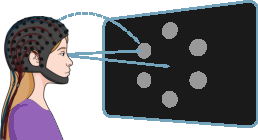
\includegraphics[width=\textwidth]{figures/covert/attention_free.pdf}
    \end{minipage}%
  }
  \end{minipage}


  \aside{
    EEG, EOG and eye-tracking
    \bigskip

    Adapted stimulation parameters
    \bigskip

    Few studies investigating abilities
    \bigskip

    Replace \textit{split} by natural \textit{free}

  }

\end{frame}


{
\setbeamercolor{background canvas}{bg=black}
\begin{frame}[c]
  \frametitle{\textcolor{white}{Eye tracking}}
  \begin{minipage}{.6\textwidth}
    \centering
    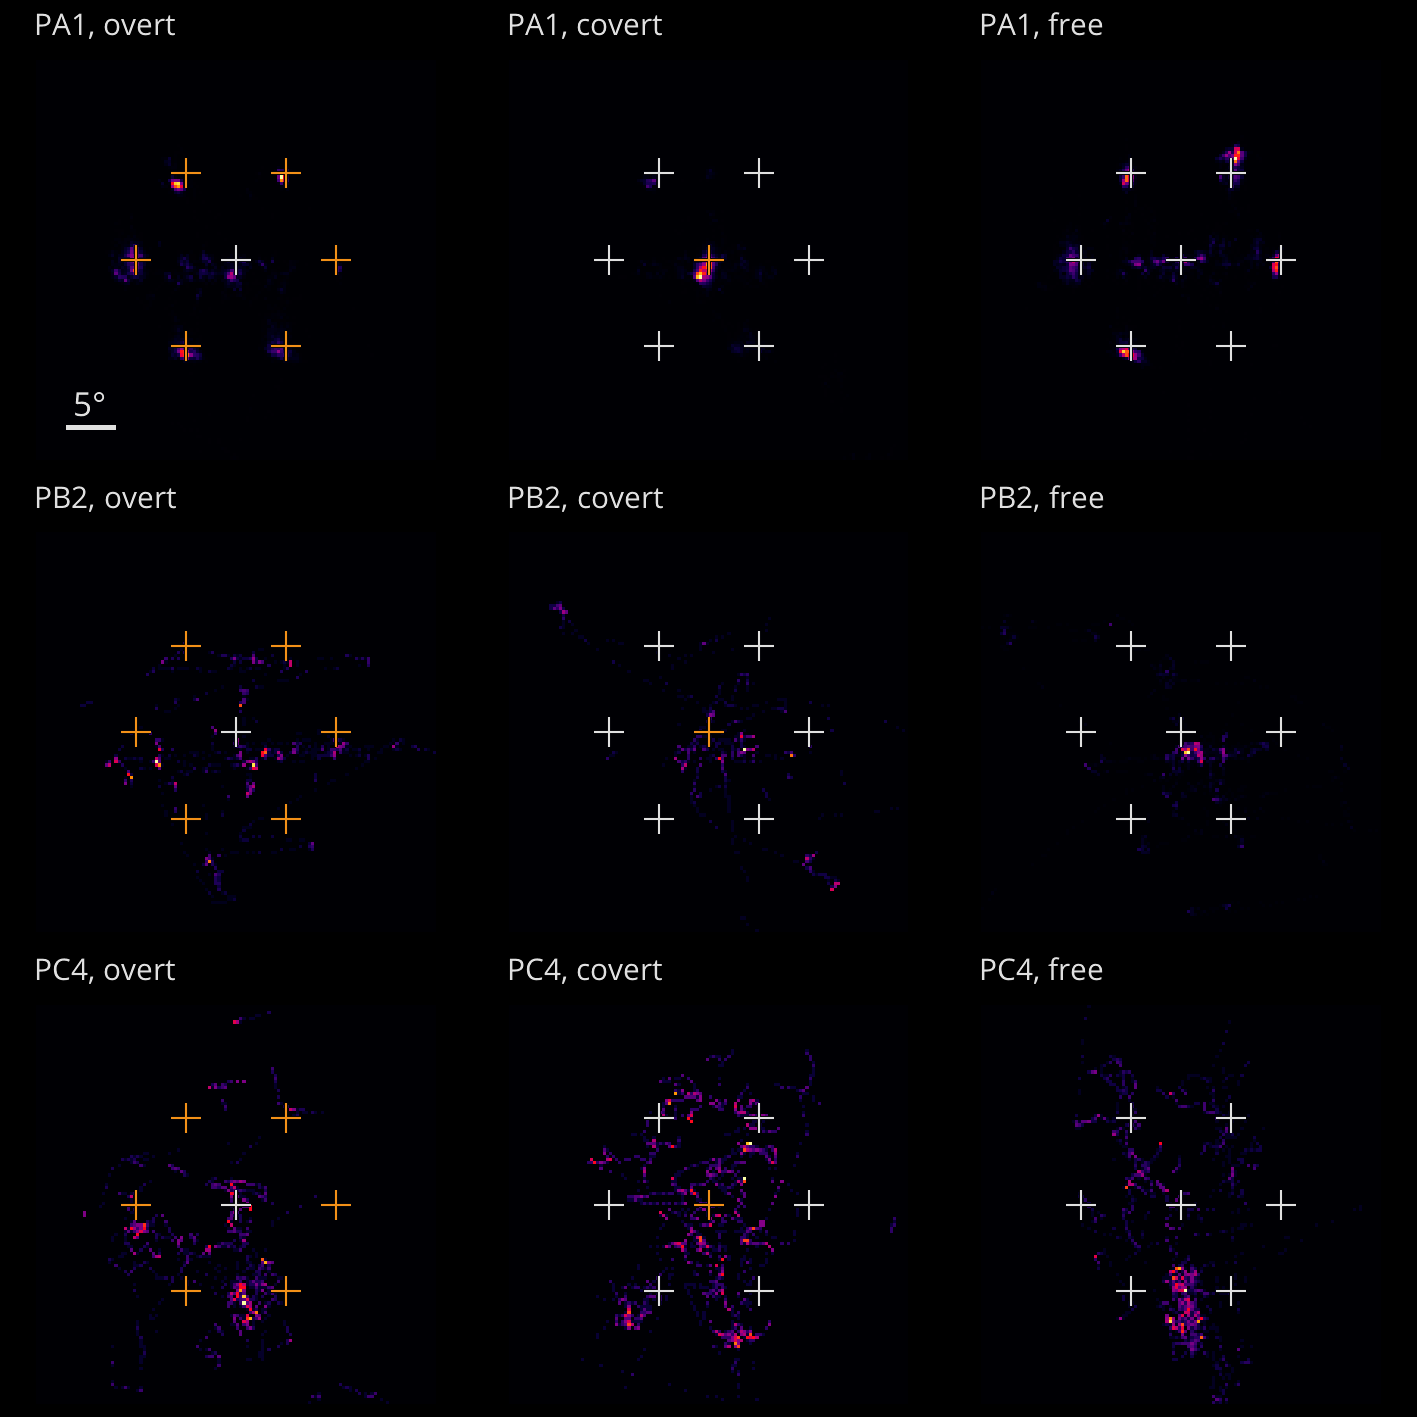
\includegraphics[width=.8\textwidth]{figures/patients/fig_gaze_defense.png}
  \end{minipage}
  \aside{
    Most used overt attention
    \bigskip
    \bigskip

    1 participant covert
    \bigskip
    \bigskip

    1 participant split
    \bigskip
    \bigskip

  }
\end{frame}
}

\begin{frame}
  \frametitle{Subject decoding performance}
  \begin{minipage}{.6\textwidth}
    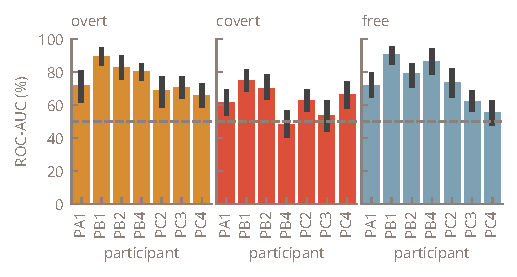
\includegraphics[width=\textwidth]{figures/patients/fig_decode.pdf}
  \end{minipage}
  \aside{
    \small
    Off-line decoder comparison,
    similar performance
    \bigskip

    Most above chance, positive effect for some
    \bigskip

    Covert lower than overt
    \bigskip

    Free not always worse
    \bigskip

    \ergo Contribution of gaze
  }
\end{frame}

\begin{frame}
  \frametitle{Recap}
  Make BCI-AT more \emph{efficient} and \emph{accessible}\\ using the \emph{visual
  ERP} paradigm
  \begin{itemize}
    \bigskip
  \item[\emph{C1:}] Decoders exploiting spatial-temporal structure
    \bigskip
  \item[\emph{C2:}] Covert attention study with healthy subjects
    \bigskip
  \item[\emph{C3:}] Decoder for eye movement independence \\ accounting for jitter
    \bigskip
  \item[\emph{C4:}] Validation with eye movement impaired subjects
  \end{itemize}
  \begin{refsection}[publications.bib]
  \aside{
    Publications
    \tiny
    \setlength{\leftmargini}{2em}
    \begin{itemize}
      \item Libert, A. et al. (2022). ``Analytic
        beamformer transformation for
        transfer learning in motion-onset
        visual evoked potential decodin''.
        en. In: \textit{Journal of Neural
        Engineering} 19.2, p. 026040.
      \item Van Den Kerchove, A. et al. (2022).
        ``Classification of Event-Related
        Potentials with Regularized
        Spatiotemporal LCMV
        Beamforming''. In: \textit{Applied Sciences}
        12.6, p. 2918.
      \item Van Den Kerchove, A. et al. (2024).
        ``Block-Term Tensor Discriminant
        Analysis for Brain-Computer
        Interfacing''. In: \textit{Journal of Neural
        Engineering.} Submitted for
        publication.
      \item Van Den Kerchove, A. et al. (2024a).
        ``Correcting for ERP latency jitter
        improves gaze-independent BCI
        decoding''. In: \textit{Journal of Neural
        Engineering.}
      \item Van Den Kerchove, A. et al.
        ``Case studies of the impact of eye
        motor impairment on visual ERP
        BCI usage''. In preparation.
    \end{itemize}
  }
  \end{refsection}
\end{frame}

\begin{frame}
    \frametitle{Conclusions}
    \begin{changemargin}
    \begin{itemize}
      \item Improved decoders enhance BCI \emph{efficiency}
      \bigskip
      \item Improvements in gaze independent decoding improve
        \emph{accessibility} for some
      \bigskip
      \item Only affects some end-user cases, need for holistic approach
      \bigskip
      \item Gained insight in requirements of BCI users with impaired eye movement
    \end{itemize}
  \end{changemargin}
\end{frame}

\begin{frame}
  \frametitle{Perspectives}
  \begin{changemargin}
    \begin{enumerate}
     \item Integrate BCI and eye-tracking \\ for impaired eye movement
     \bigskip
     \item On-line experiments
     \bigskip
     \item User-centered design study
     \bigskip
     \item Models capturing multi-component and
       non-stationary aspect of (covert) ERPs
  \end{enumerate}
  \end{changemargin}
\end{frame}

\outline{Q\&A}{figures/qa.pdf}
%
%%% BACKUP Slides ==============================================================



\begin{frame}[noframenumbering]
  \frametitle{Experimental procedure \\ CVSA-ERP}
  hardware, locations, timings, nr of blocks, ...
\end{frame}
\begin{frame}
  \frametitle{Experimental procedure \\ end-user study}
  hardware, locations, timings, nr of blocks, ...
\end{frame}

\begin{frame}[noframenumbering]

  \frametitle{Block-term tensor discriminant analysis procedure}
  backward model image and equation

  forward model image and equation

  deflation image and equations

  model selection procedure
\end{frame}

\begin{frame}[noframenumbering]

  \frametitle{Block-term tensor discriminant analysis procedure}
  backward model image and equation

  forward model image and equation

  deflation image and equations

  model selection procedure
\end{frame}

\begin{frame}[noframenumbering]
 WCBLE training procedure
\end{frame}

\begin{frame}[noframenumbering]
  WCBLE test procedure
\end{frame}

\begin{frame}[noframenumbering]
  \frametitle{Subjects with physical, speech and gaze impairment}

  \begin{tabular}{@{}l|lrlrl@{}}
      \textbf{ID}  & \textbf{Diagnosis} & \textbf{Age} &
      \textbf{Speech} & \textbf{Trach.} & \textbf{Communication} \\ \hline
      PA1 & bulbar-onset ALS & 58  & absent  & no          & tablet                 \\
      PB1 & Friedreich's ataxia & 41  & impaired & no          & verbal                 \\
      PB2 & Friedreich's ataxia & 43  & impaired & no          & verbal                 \\
      PB4 & Friedreich's ataxia & 48  & impaired & no          & verbal                 \\
      PC2 & brainstem stroke & 43  & absent  & yes         &  eye movement \\
      PC3 & brainstem stroke & 43  & absent  & yes         & letterboard            \\
      PC4 & cerebellar stroke & 54  & absent  & yes         & letterboard \\
  \end{tabular}

\end{frame}



\begin{frame}[noframenumbering]
  \frametitle{Visual skill and eye movement impairment}
  \newcommand{\skill}{}
  \newcommand{\noskill}{x}
  \newcommand{\snoskill}{o}

  \begin{tabular}{l|ccccccc}
                            & PA1      & PB1      & PB2       & PB4      & PC2       & PC3       & PC4 \\ \hline
    \small Visual fixation         & \noskill & \noskill & \noskill  & \noskill & \noskill  & \noskill  & \noskill \\
    \small Eyelid function         & \skill   & \skill   & \skill    & \skill   &  \skill  & \noskill  & \noskill \\
    \small Ocular motility         & \skill   & \noskill & \skill    & \noskill & \snoskill & \snoskill & \noskill\\
    \small Binocular vision        & \skill   & \skill   & \skill    & \skill   & \noskill  & \snoskill & \snoskill \\
    \small Field of vision         & \skill   & \skill   & \skill    & \skill   & \skill    & \noskill  & \noskill \\
    \small Involuntary movement    & \skill   & \noskill & \snoskill  &
    \noskill &  \noskill  & \noskill  & \skill \\ \hline
  Visual acuity (logMAR)  & 0.0      & 0.0      & 0.6       & 0.2      & 0.0       & 0.7  & 0.6\\
  \end{tabular}
  \bigskip

  x: impaired, o: severely impaired
\end{frame}


\begin{frame}[c, noframenumbering]
\frametitle{User-Centered Design}

  \begin{minipage}[c]{.5\textwidth}
  \begin{tabular}{|l|l|}
    \hline
     & \emph{Principles} \\ \hline
     \emph{P1} & understand user, task, environment \\
     \emph{P2} & early and active user involvement \\
     \emph{P3} & driven by user-centered evaluation \\
     \emph{P4} & iterative design \\
     \emph{P5} & adress holistic experience \\
     \emph{P6} & multidisciplinary design \\
    \hline
  \end{tabular}
  \end{minipage}\hfill%
  \begin{minipage}[c]{.4\textwidth}
  \end{minipage}

\end{frame}


\end{document}
